% arara: lualatex: { shell: yes, action: nonstopmode, synctex: yes}
% arara: lualatex: { shell: yes, action: nonstopmode, synctex: yes}
% asarara: lualatex: { shell: yes, action: nonstopmode, synctex: yes,  options: "-output-directory=_build"}
% asarara: lualatex: { shell: yes, action: nonstopmode, synctex: yes,  options: "-output-directory=_build"}
\documentclass[landscape]{article}
\usepackage[ngerman]{babel}
\usepackage[no-math]{fontspec}

\usepackage{mwe}
\usepackage{luacode}
\usepackage{shellesc}
% \documentclassw[11pt, a4paper,ngerman]{article}
\usepackage{basicff}

\usetikzlibrary{patterns} % preamble
\tcbuselibrary{skins} % preamble

\usepackage{tikz}
% \usepackage{PTSansNarrow}
\usetikzlibrary{matrix}

\usepackage{pgfplots}
\pgfplotsset{
 compat=newest
  }
\tcbset{colframe=red!75!black}
\newenvironment{proggen}{\begin{center}}{\end{center}}

\usepackage{array}
% \setmainfont[Path=/Applications/Microsoft Word.app/Contents/Resources/Fonts/]{Calibri.ttf}
% \setsansfont[Path=/Applications/Microsoft Word.app/Contents/Resources/Fonts/]{Calibri.ttf}
% \setmonofont[Path=/Applications/Microsoft Word.app/Contents/Resources/Fonts/]{Calibri.ttf}
% \usepackage{datetime}
% \pagestyle{fancy}


\setmainfont{UbuntuL.ttf}
\setsansfont{UbuntuR.ttf}
\setmonofont{UbuntuMonoR.ttf}

\newcolumntype{C}[1]{>{\centering\arraybackslash}m{#1}}

\oddsidemargin-10mm
\title{
\color{white}
 $\bullet$ \\ $\bullet$ \\ $\bullet$ \\
 \color{black}
 % \color{white}
 % $\bullet$ \\
 \color{black}
 NOP \\
Luatex \\
\color{white}
$\bullet$ \\
\color{black}
 \begin{center}
	% \includegraphics[scale=0.5]{./pictures/CaptainWarschburger.jpg}
\end{center}
 % \includegraphics{./pictures/wohnzimmer.png}
}
% \includegraphics{./pictures/asrock.png} Q1900M \\ \color{white} $\bullet$ \\ $\bullet$ \\ $\bullet$ \\ \color{black} \\ \apple \\ 10.10.3

\author{Daniel Krah}
% \rfoot{Compiled on \today\ at \currenttime}
% \cfoot{}
% \lfoot{Page \thepage}
% \date{1.6.2015}

\begin{document}
\AddToShipoutPicture{\BackgroundPic}
\maketitle%
\newpage%
 % \tableofcontents%
% \newpage
%==================================================================================
% \begin{center}
% \textbf{Vorwort}
% \end{center}



%
% \input{hardware.tex}







%  To Do
% \input{todo.tex}
\newpage
% \section{Überblick}


% \begin{displaymath}
%   E = \frac{m_{0} c^{2}}{\sqrt{1-v^{2}/c^{2}}}
% \end{displaymath}

% \begin{luacode}
%   for x=1,600 do
%     tex.print(x+2)
%   end
% \end{luacode}
\section{Warum \LaTeX \  bzw. LUA\TeX ?}
\subsection{Vorteile von \LaTeX}
\begin{itemize}
  \item Tex Dateien kann man auch noch nach Jahren öffnen \\und in der Regel auch übersetzen.
  \item Keine Binärdateien. (Dokument auf Github direkt lesbar)
  \item Einfaches zusammenarbeiten (merge problemlos möglich)
  \item Nutzung mit Github und Travis CI relativ einfach
\end{itemize}
\subsection{Warum dann LUA\TeX ?}
\begin{itemize}
  \item Unterstützung von True-Type-Schriften \\(KEIN Zugriff auf Systemschriften !!!)
  \item komplexeres Programmieren innerhalb von Tex möglich.
\end{itemize}


\section{Warum GitHub und Travis-CI ?}

Im Prinzip könnte man jeden x beliebigen Server ... \\
Dort: \\
ein Git Repo + ssh und ein CI System. \\

Man könnte eines selbst zu Hause hosten und hätte die volle Kontrolle.\\

ABER:
Als Student möchte man vielleicht in Gruppen zusammen arbeiten um sich zusammen eine Mitschrift anzufertigen.
Nicht jeder möchte sich eine komplette \LaTeX - Installation an tun.\\

\"{}Och ne, iss mir zuviel Uffriss ...\"{} \\

Durfte ich mir schon oft anhören.






% \begin{itemize}
%   \item Tex Dateien kann man auch noch nach Jahren öffnen \\und in der Regel auch übersetzen.
%   \item Keine Binärdateien. (Dokument auf Github direkt lesbar)
%   \item Einfaches zusammenarbeiten (merge problemlos möglich)
%   \item Nutzung mit Github und Travis CI relativ einfach
% \end{itemize}
% \subsection{Warum dann LUA\TeX ?}
% \begin{itemize}
%   \item Unterstützung von True-Type-Schriften \\(KEIN Zugriff auf Systemschriften !!!)
%   \item komplexeres Programmieren innerhalb von Tex möglich.
% \end{itemize}

% 
\newpage

\section{Github + Travis CI - \ \  \"{} the pdflatex way \"{}}
\subsection{Was wird benötigt ?}
{\color{green}Kostenlose} Variante (nur public Repo's):
\begin{itemize}
  \item Ein Github - Account
  \item Ein Travis-CI (.org) Account
  \item Das Travis Command-line Tool
\end{itemize}
\vspace{0.5cm}
{\color{red}Kostenpflichtige} / Studenten Variante \\(Auch private Repo's / und sofortige build's):
\begin{itemize}
  \item Ein kostenpflichtiger Github - Account ( \$7/ Monat)
  \item Ein kostenpflichtiger Travis-CI (.com) Account ( \$69/ Monat)
  \item Alternativ ein Student Developer Pack von Github \\ siehe: https://education.github.com/pack
  \item Das Travis Command-line Tool
\end{itemize}


%
%   Seite 4
%
%   Github
%
\newpage
\subsection{Einrichtung}
\subsection{Github}
Als erstes benötigen wir einen Github Account inkl. Repo.
\begin{center}
  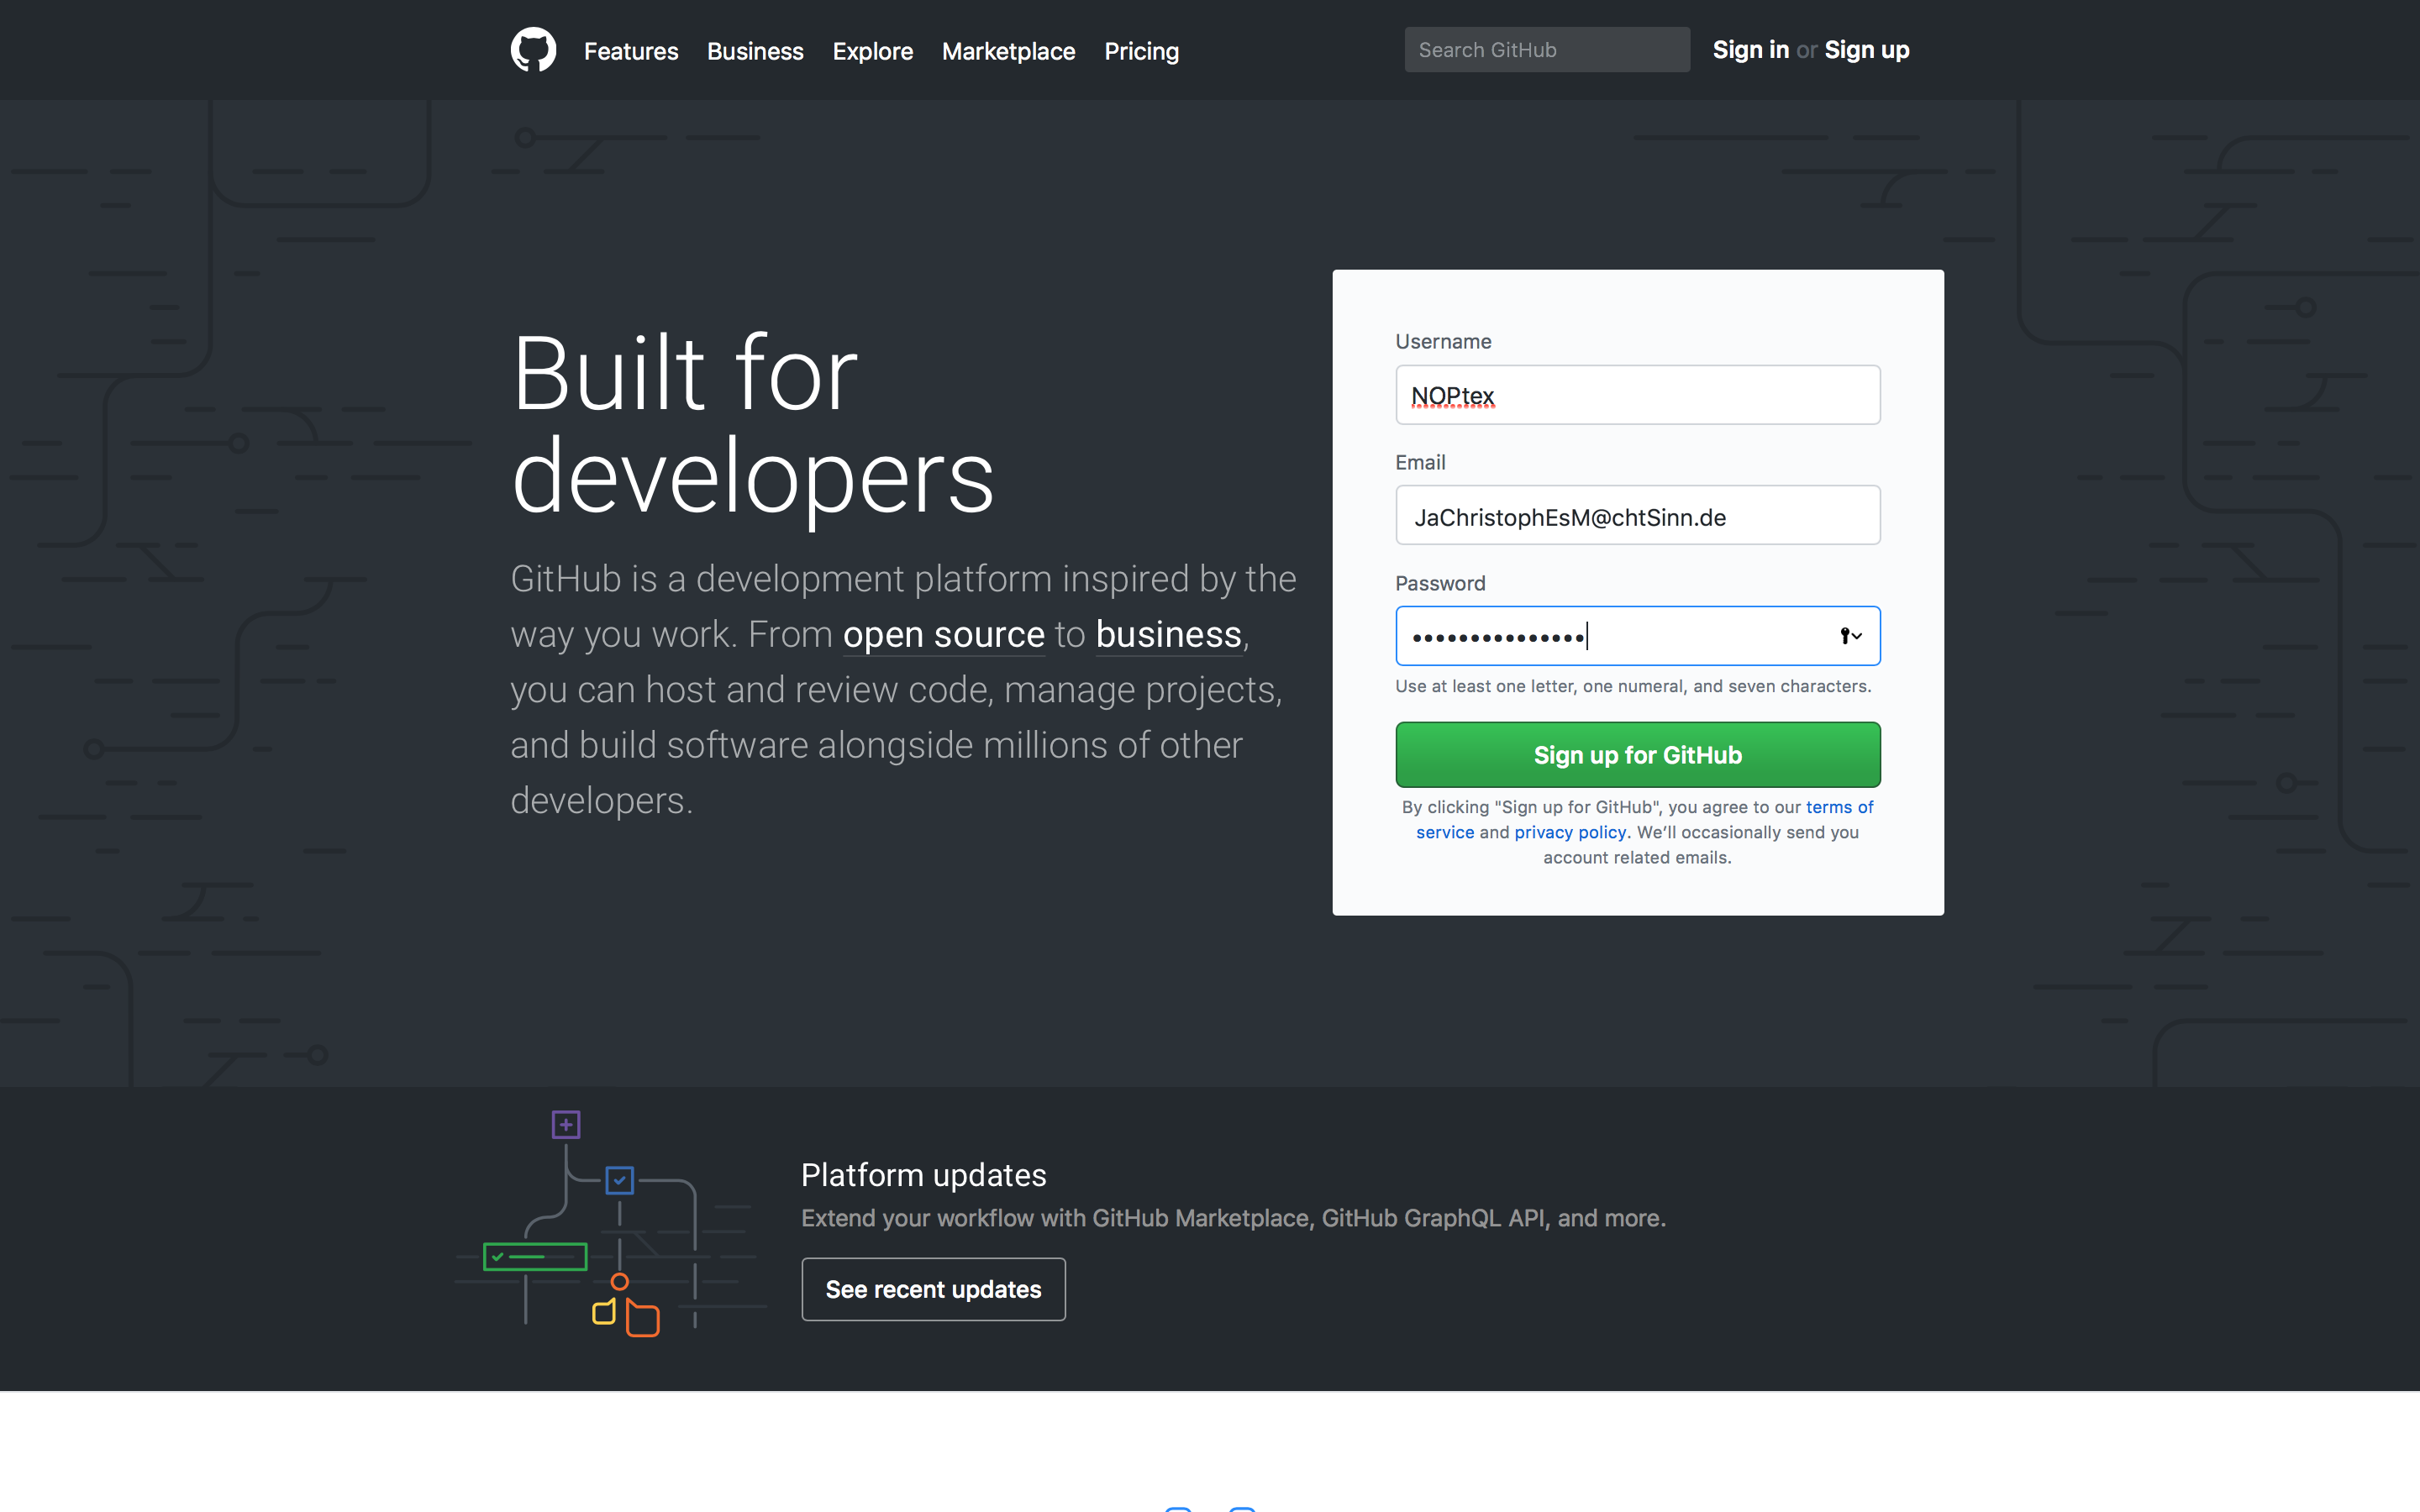
\includegraphics[trim = 300px 10px 300px 0px, clip,height=11cm]{./bilder/1Github.png}
\end{center}

% "l, b, r, t"
% \begin{figure}
% 	\centering
% \end{figure}\includegraphics[trim = 20px 10px 20px 30px, clip, width=\textwidth]{Beispiel.jpg}
% 	\caption{Hier steht der Beschriftungstext.}
% 	\label{fig:Beispiel}
% \end{figure}



\newpage
(Im Verlauf dieses Vortrages verwende ich:\\

https://github.com/NOPtex/NOP)\\


Dort befindet sich ein funktionierender Prototyp. \\
(Welcher aber noch ein paar zusätzlich Dateien beinhaltet.) \\

Prinzipiell reicht eine \TeX -Datei und die .travis.yml.

\begin{center}
  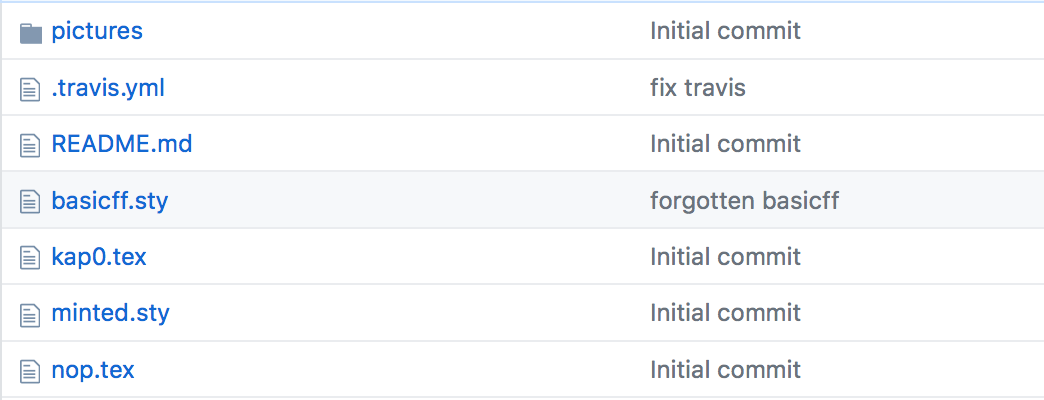
\includegraphics[width=0.8\textwidth]{./bilder/2Boilerplate.png}
\end{center}

%
%
% \vspace{0.5cm}
%
% \begin{center}
%   \includegraphics[width=1.0\textwidth]{./bilder/plainRepo.png}
% \end{center}

%
%   Seite 5
%
%   Github
% \cleardoublepage

\newpage % ============================================= Newpage ===================


\begin{figure}[ht]
  \subsection{Travis CI}
  \subsubsection{In Travis CI einloggen und mit Github verbinden}
\adjustbox{valign=t}{\begin{minipage}[t]{0.50\textwidth}
\begin{framed}
  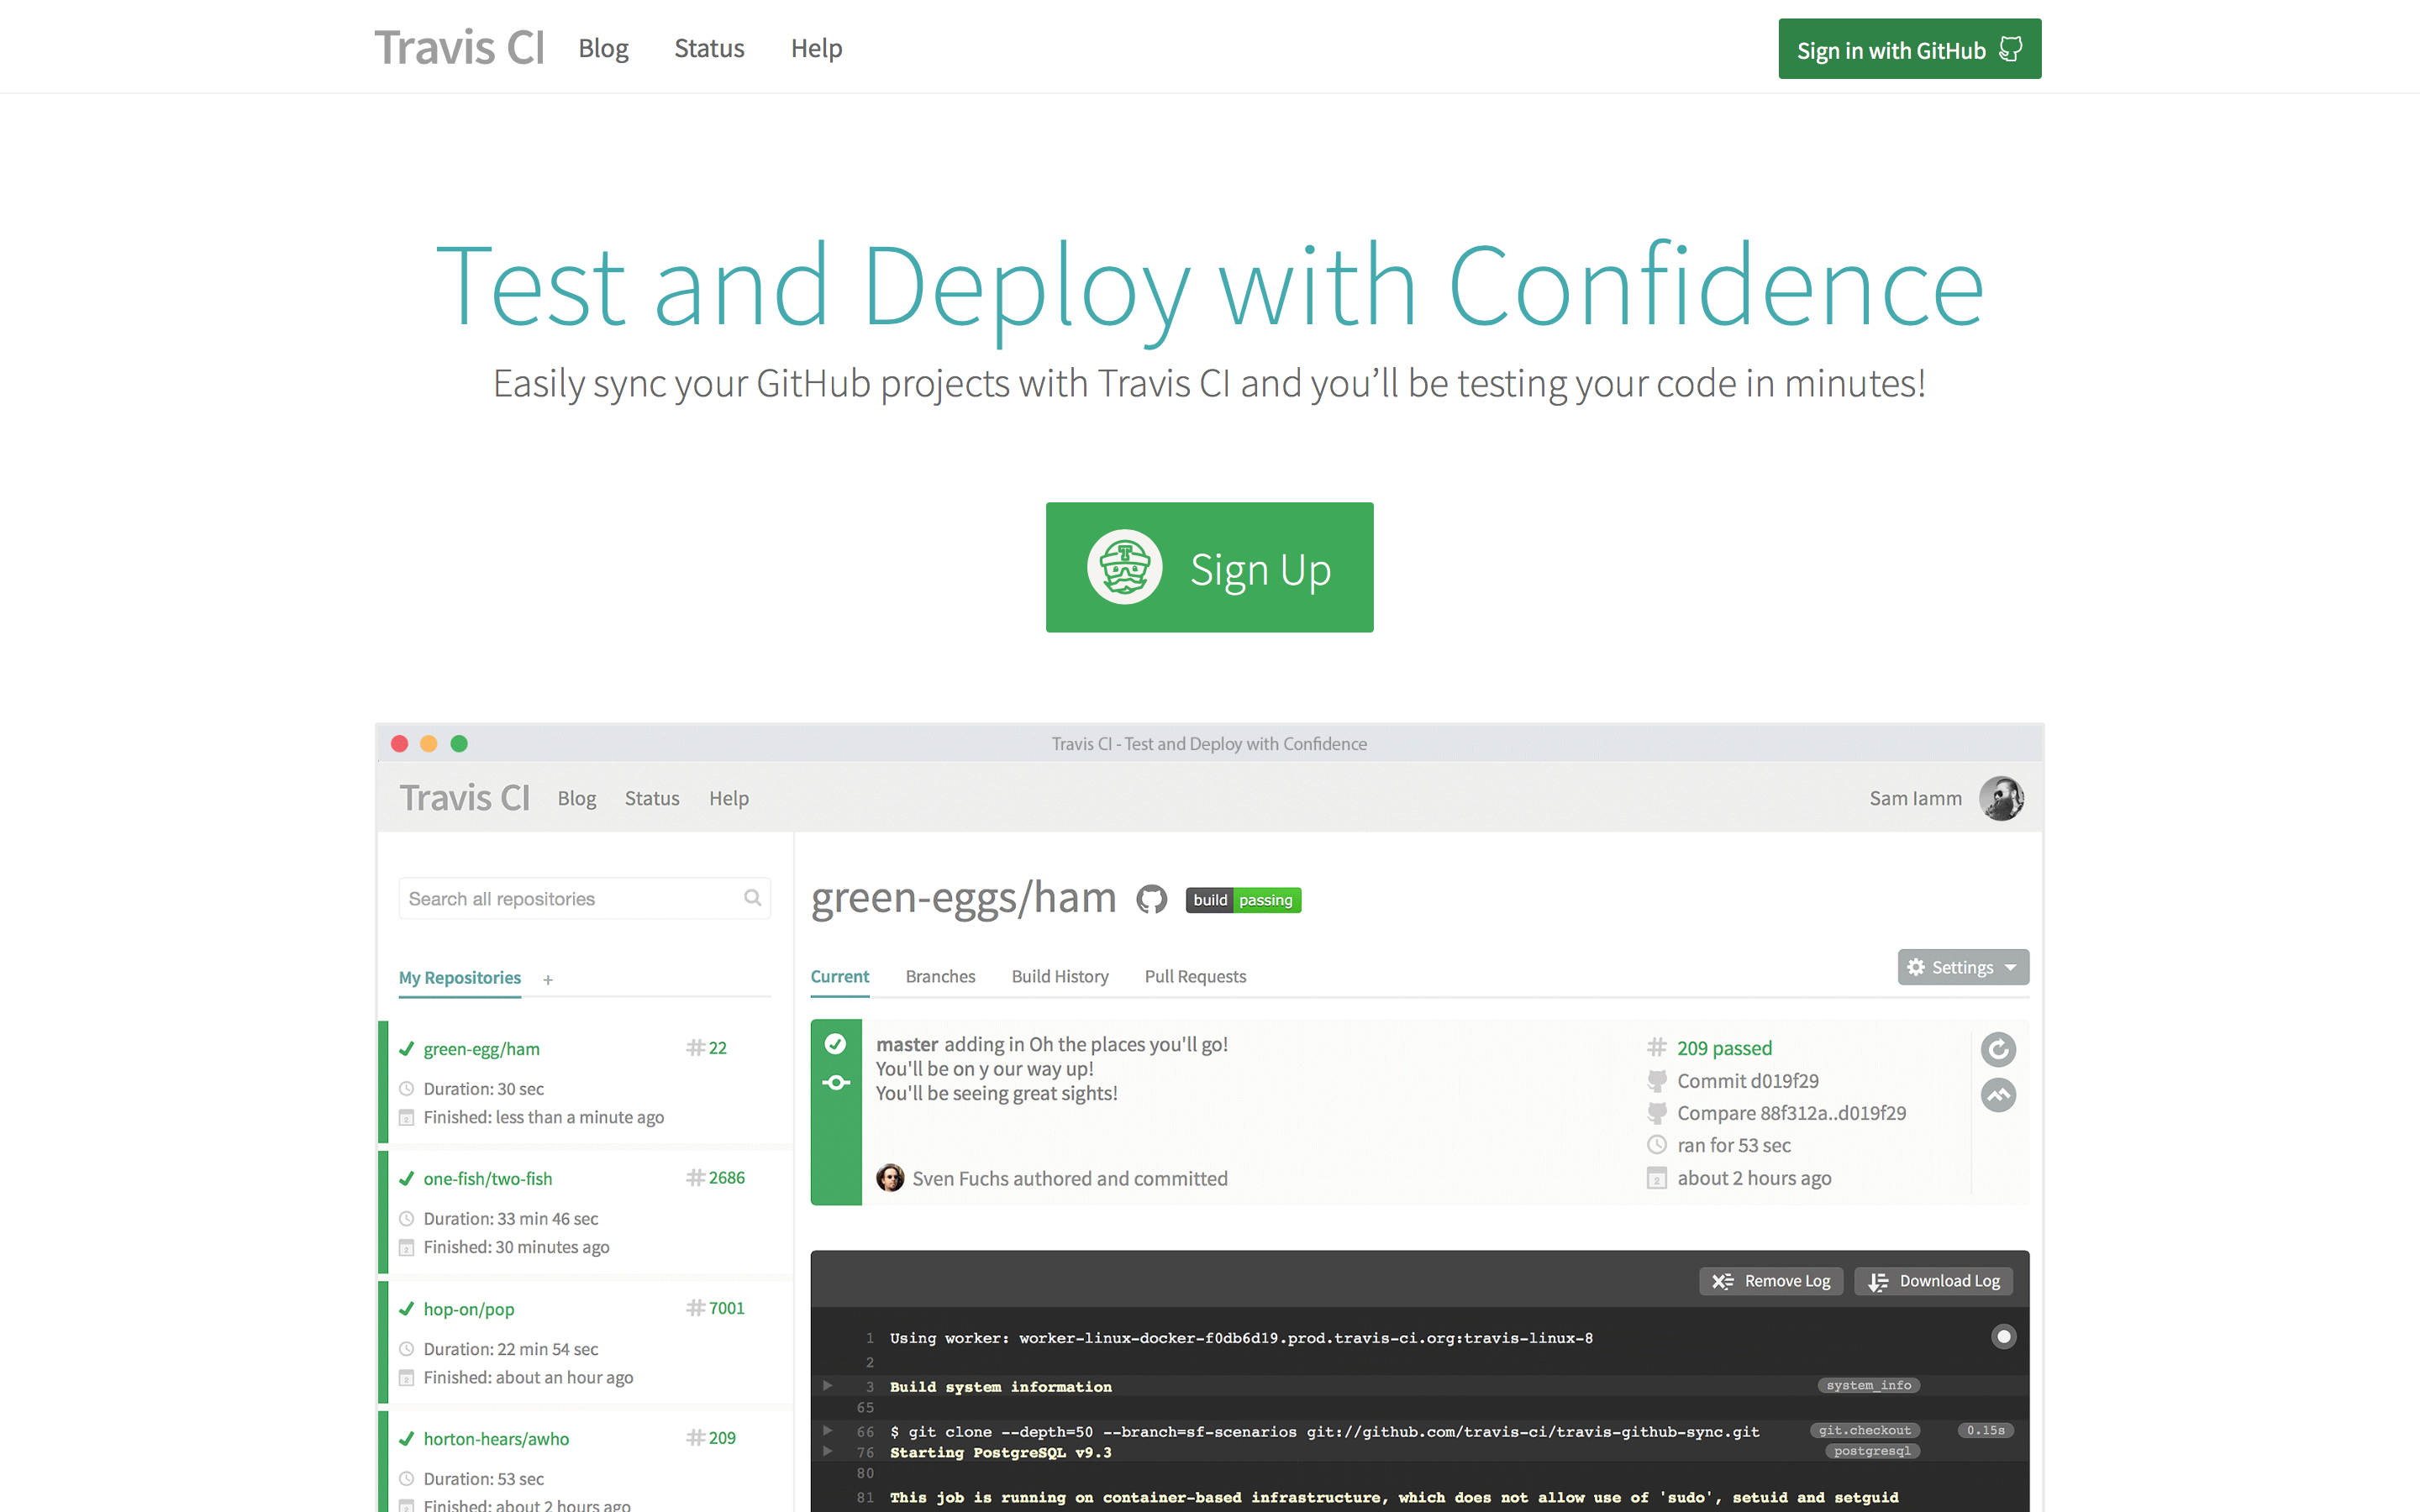
\includegraphics[width=1.0\textwidth]{./bilder/3travisSignUP.png}
\end{framed}

\end{minipage}}
% \hfill
\adjustbox{valign=t}{\begin{minipage}[t]{0.45\textwidth}
\vspace{0pt}
\huge
Da Travis nur mit Github \\funktioniert ist die Einrichtung recht \"{}trivial\"{}.
% \caption{Kapazität}
\end{minipage}}
% \end{figure}
% \vspace{0.5cm} % ----------------------------------- vspace
% \begin{figure}[ht]
\adjustbox{valign=t}{\begin{minipage}[t]{0.50\textwidth}
% \vspace{0.5cm}
\begin{framed}
  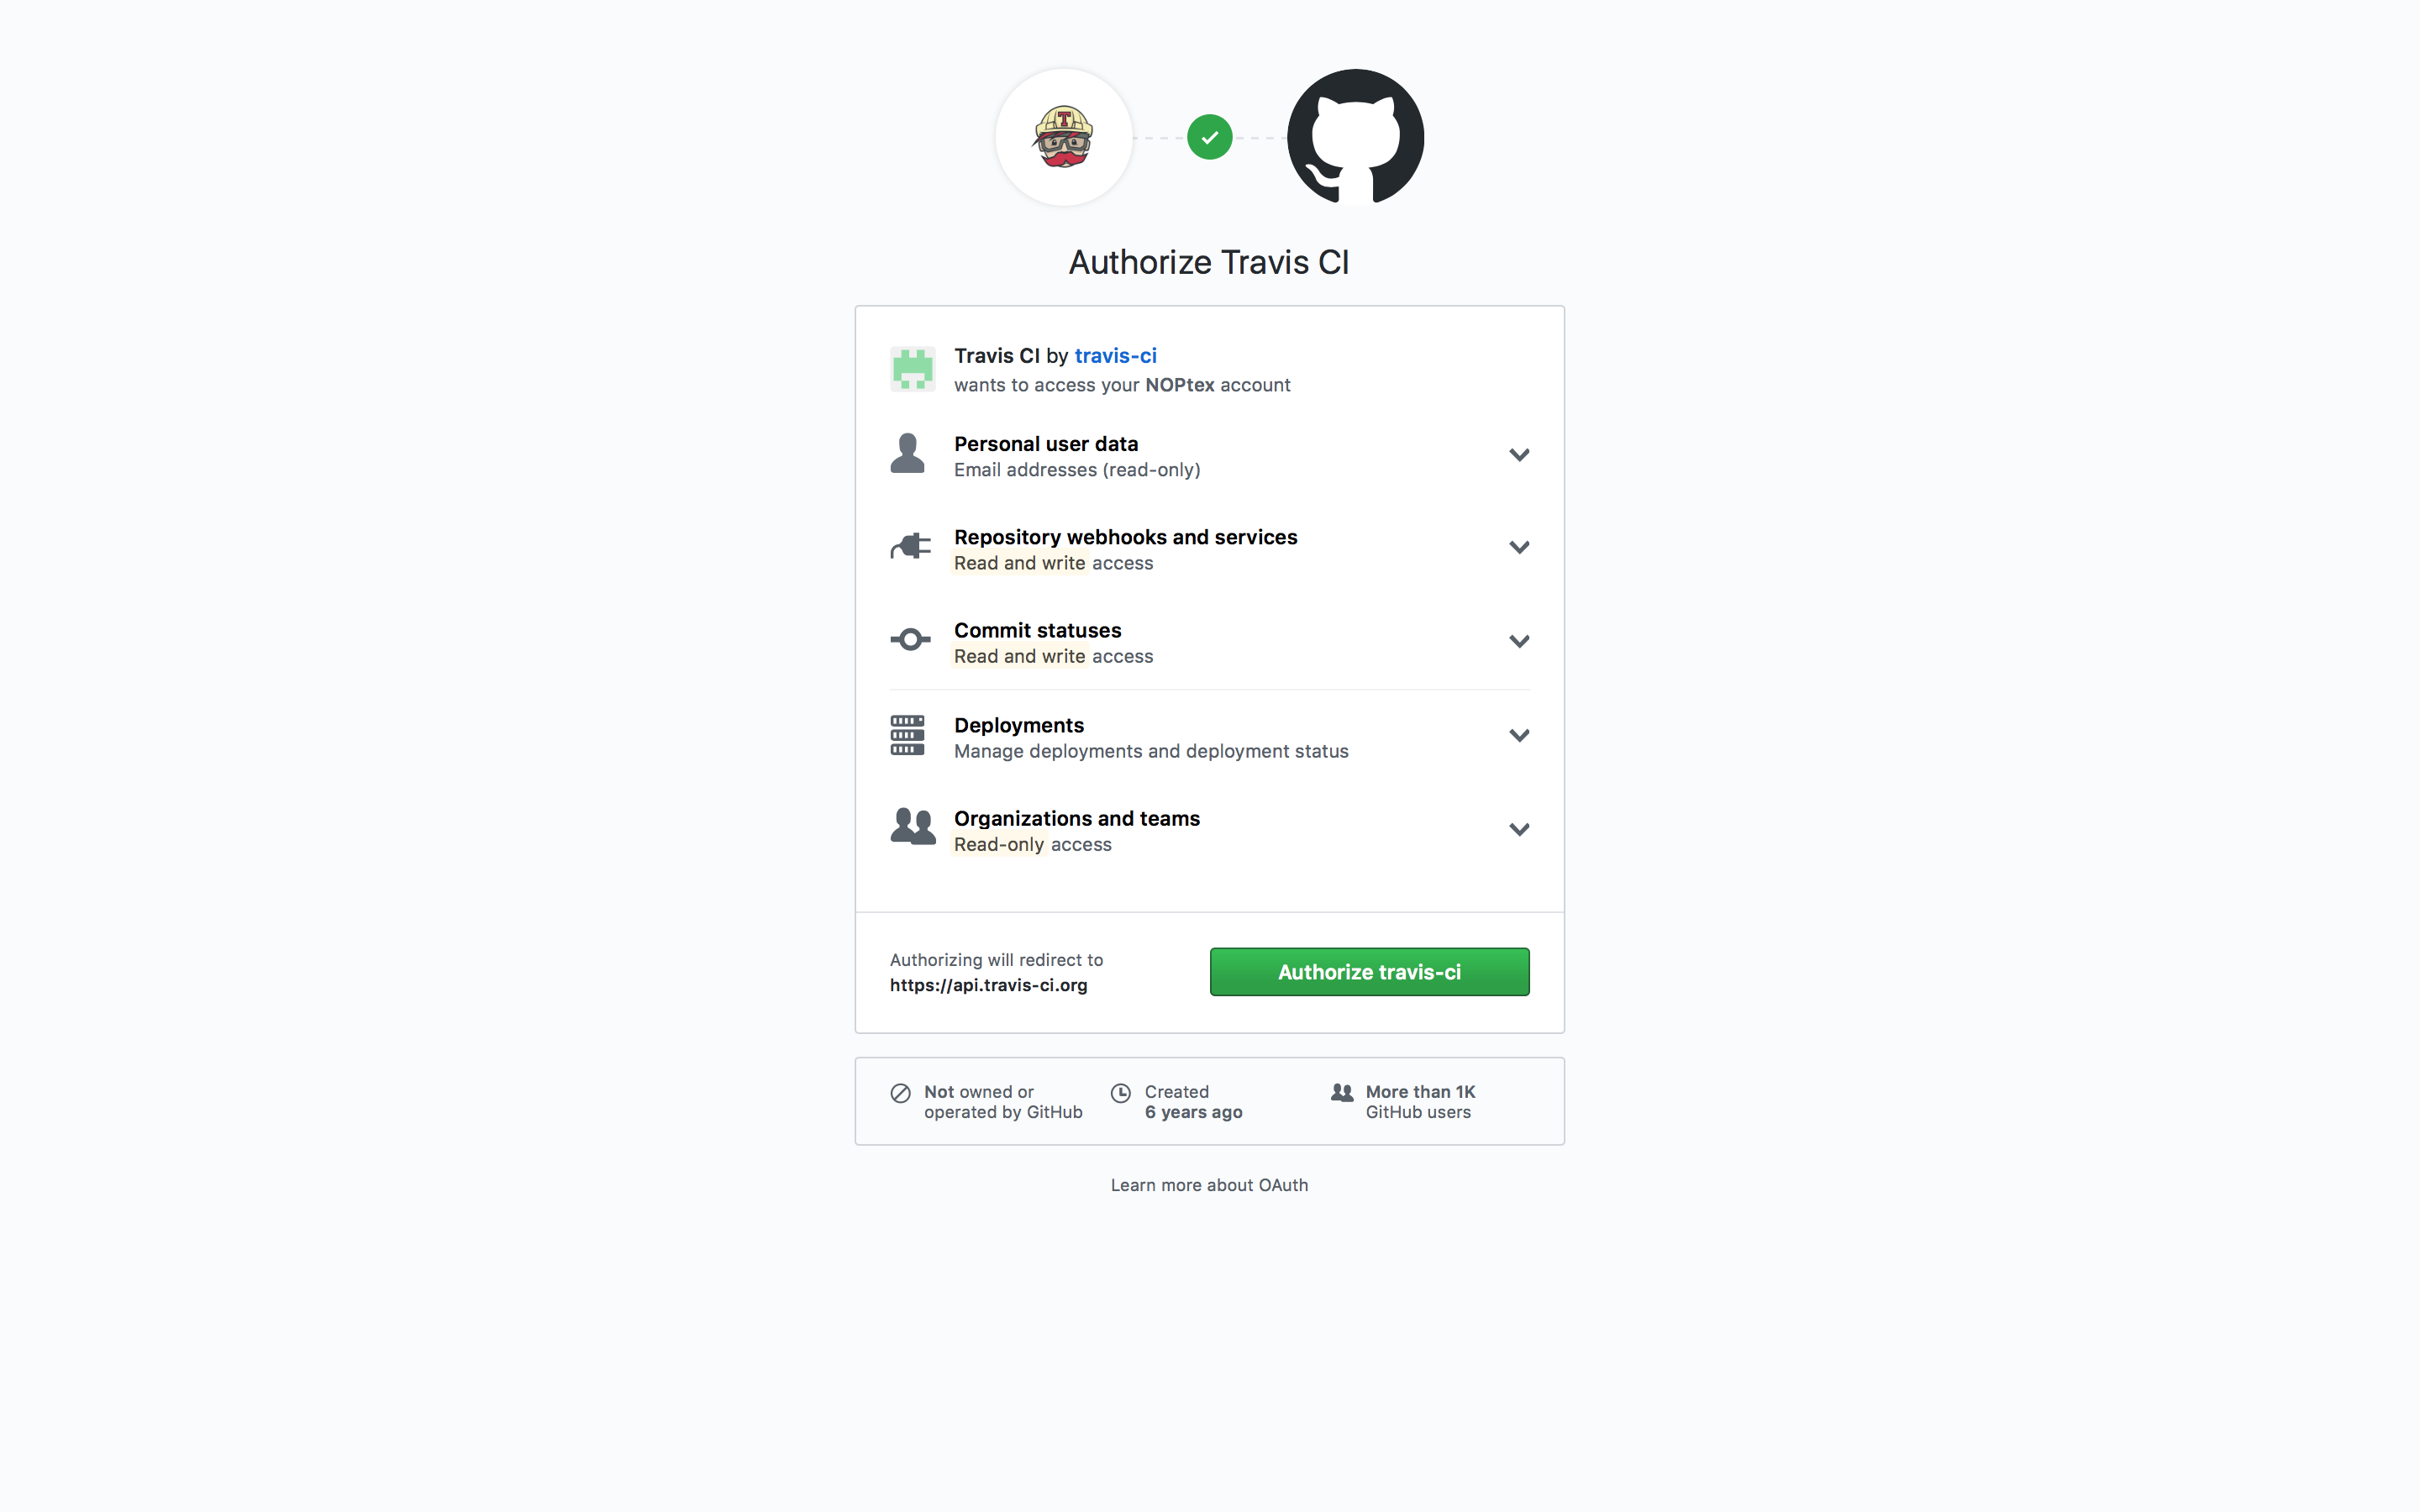
\includegraphics[width=1.0\textwidth]{./bilder/4TRAVISauthGITHUB.png}
\end{framed}

\end{minipage}}
\hfill
\adjustbox{valign=t}{\begin{minipage}[t]{0.45\textwidth}
\vspace{0pt}
\huge
Travis benötigt einige \\Berechtigungen welche man in diesem Schritt erteilt.
% \caption{Kapazität}
\end{minipage}}
\end{figure}

\clearpage % GleitObjekte anzeigen






\newpage % ============================================= Newpage ===================


\begin{figure}[ht]
  \subsubsection{Github - Repo aktivieren}
\adjustbox{valign=t}{\begin{minipage}[t]{0.50\textwidth}
\begin{framed}
  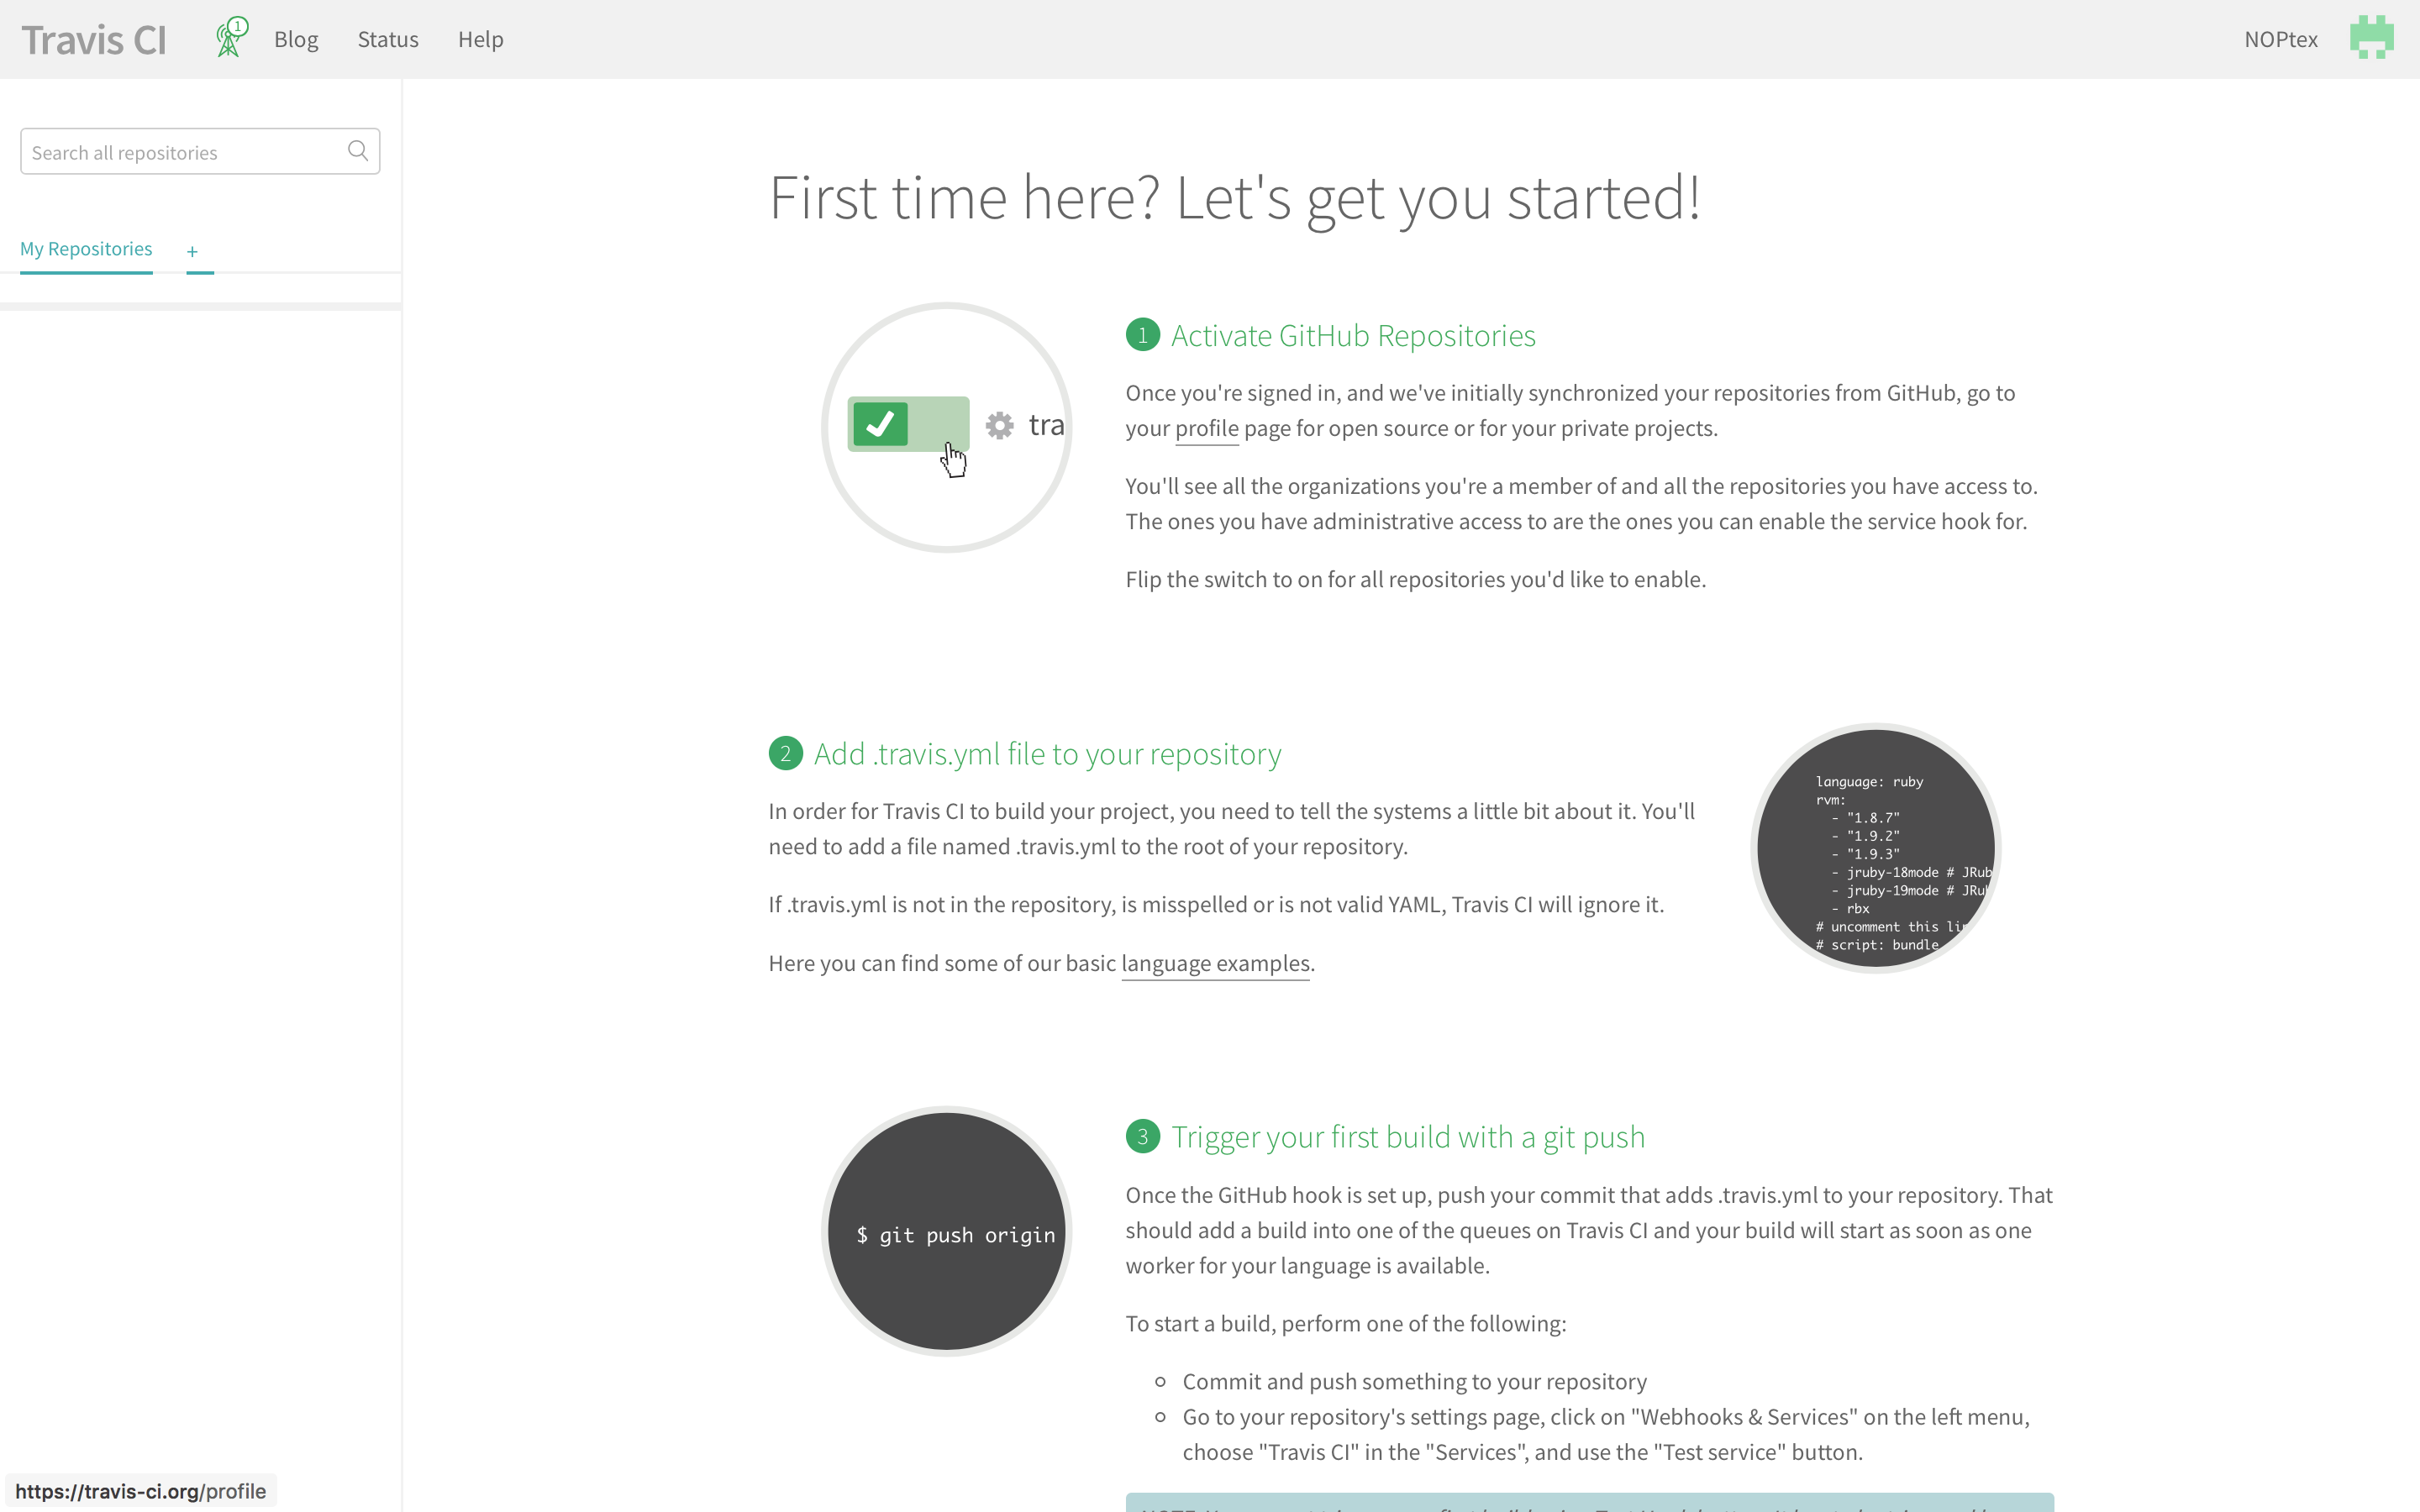
\includegraphics[width=1.0\textwidth]{./bilder/5TRAVISfirstSignIn.png}
\end{framed}

\end{minipage}}
% \hfill
\adjustbox{valign=t}{\begin{minipage}[t]{0.45\textwidth}
\vspace{0pt}
\huge
Da Travis nur mit Github funktioniert ist die Einrichtung recht einfach.
% \caption{Kapazität}
\end{minipage}}
% \end{figure}
% \vspace{0.5cm} % ----------------------------------- vspace
% \begin{figure}[ht]
\adjustbox{valign=t}{\begin{minipage}[t]{0.50\textwidth}
% \vspace{0.5cm}
\begin{framed}
  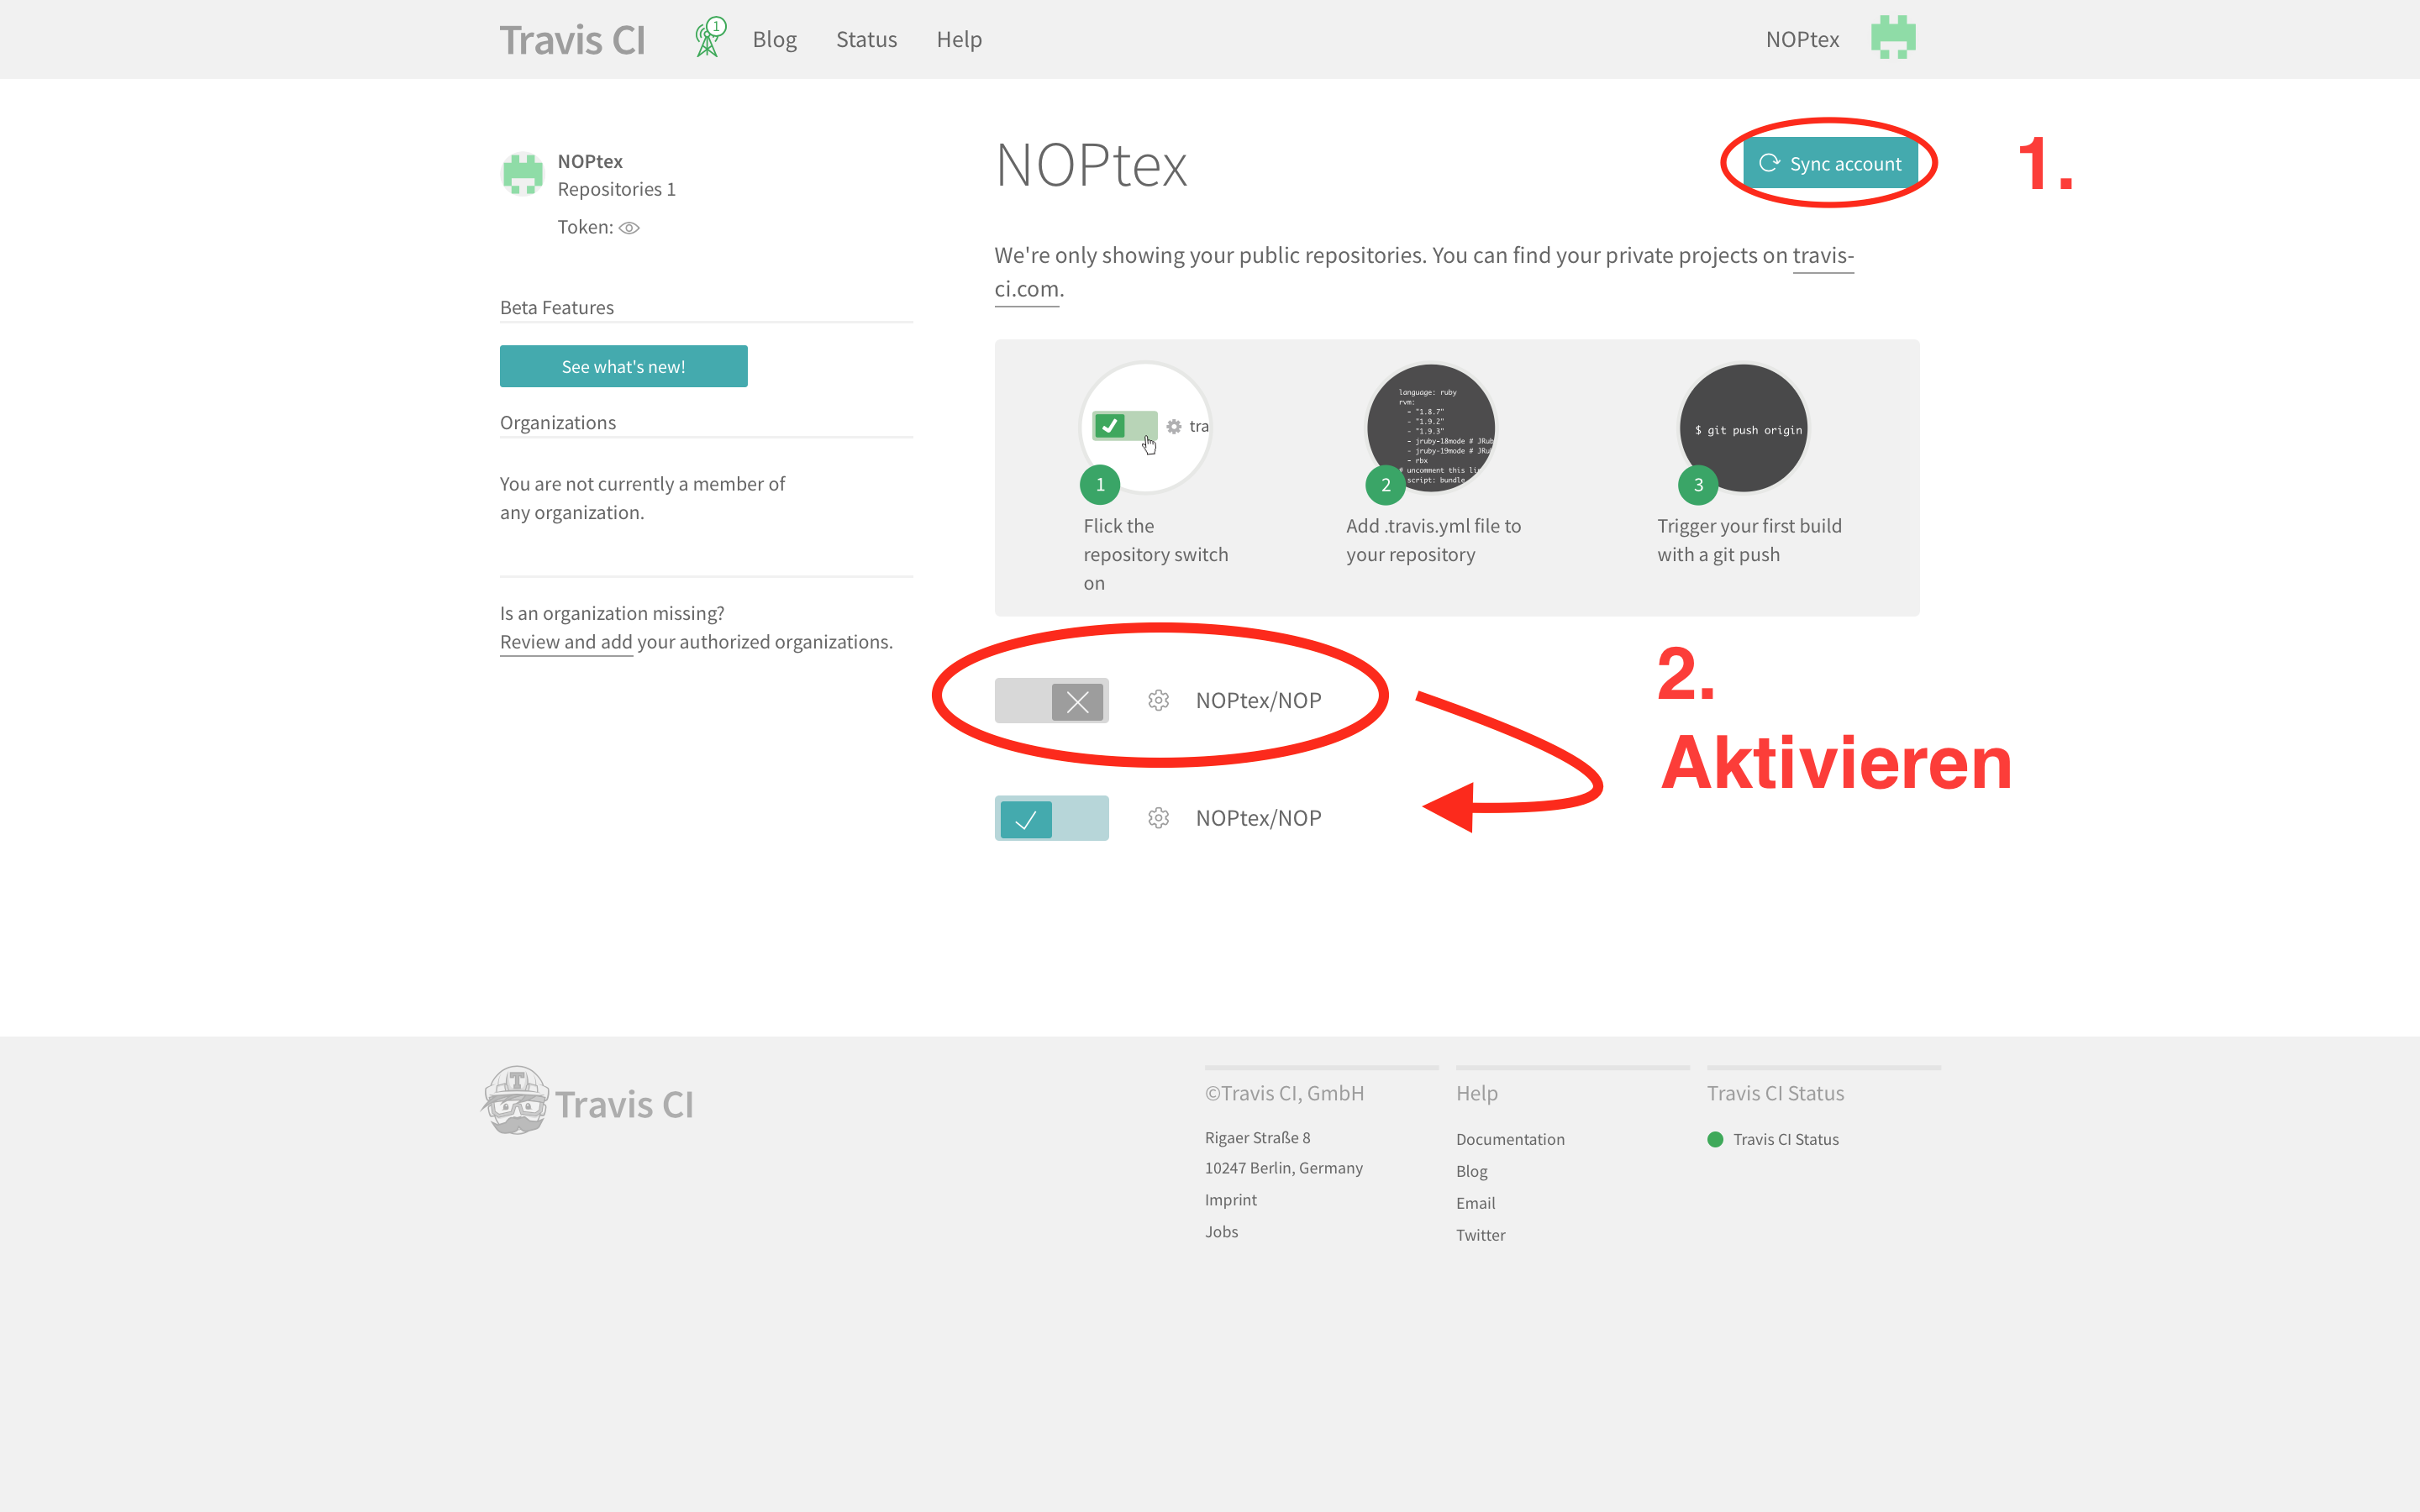
\includegraphics[width=1.0\textwidth]{./bilder/6TRAVISActivateREPO.png}
\end{framed}

\end{minipage}}
\hfill
\adjustbox{valign=t}{\begin{minipage}[t]{0.45\textwidth}
\vspace{0pt}
\huge
Travis benötigt einige Berechtigungen welche man im nächsten Schritt erteilt.
% \caption{Kapazität}
\end{minipage}}
\end{figure}

\clearpage % GleitObjekte anzeigen


\newpage % ============================================= Newpage ===================


\begin{figure}[ht]
  \subsubsection{Build-Einstellungen setzen}
\adjustbox{valign=t}{\begin{minipage}[t]{0.50\textwidth}
\begin{framed}
  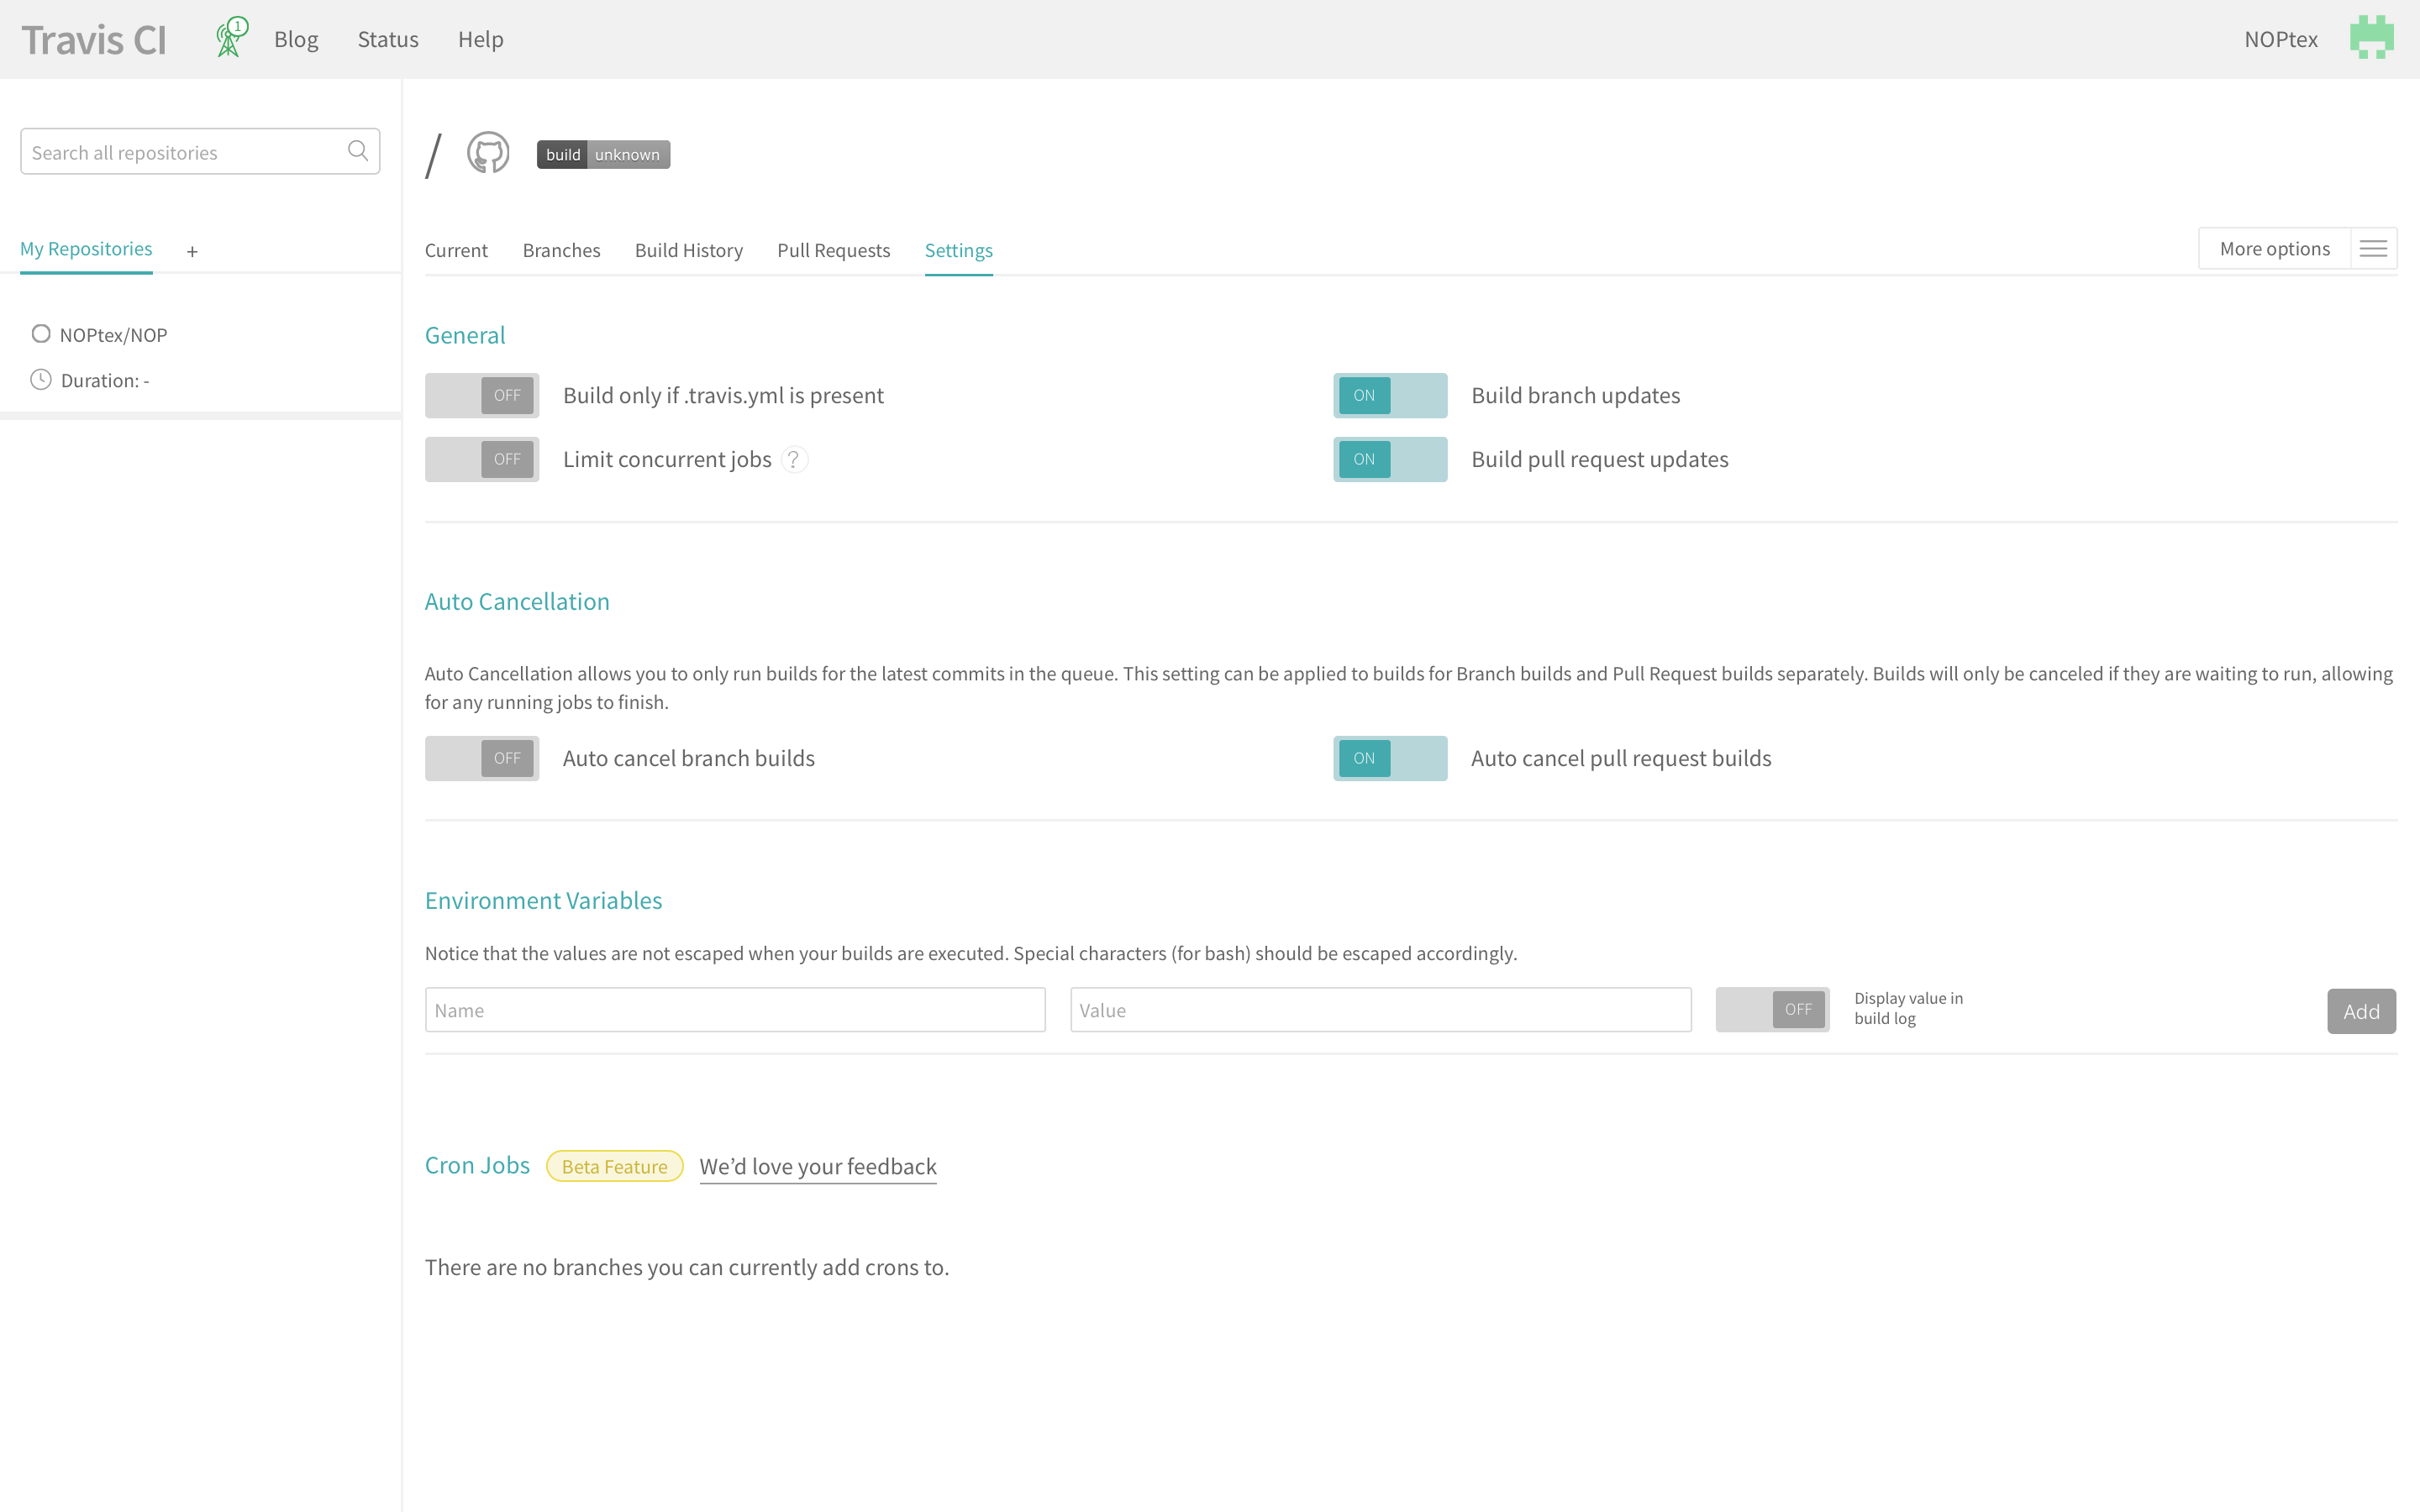
\includegraphics[width=1.0\textwidth]{./bilder/7TRAVISOptionsbase.png}
\end{framed}

\end{minipage}}
% \hfill
\adjustbox{valign=t}{\begin{minipage}[t]{0.45\textwidth}
\vspace{0pt}

\includegraphics[width=1.0\textwidth]{./bilder/7_1REPOsettings.png}
\huge
Über das Zahnrad kommt man zu den Einstellungen.
% \caption{Kapazität}
\end{minipage}}
% \end{figure}
% \vspace{0.5cm} % ----------------------------------- vspace
% \begin{figure}[ht]
\adjustbox{valign=t}{\begin{minipage}[t]{0.50\textwidth}
% \vspace{0.5cm}
\begin{framed}
  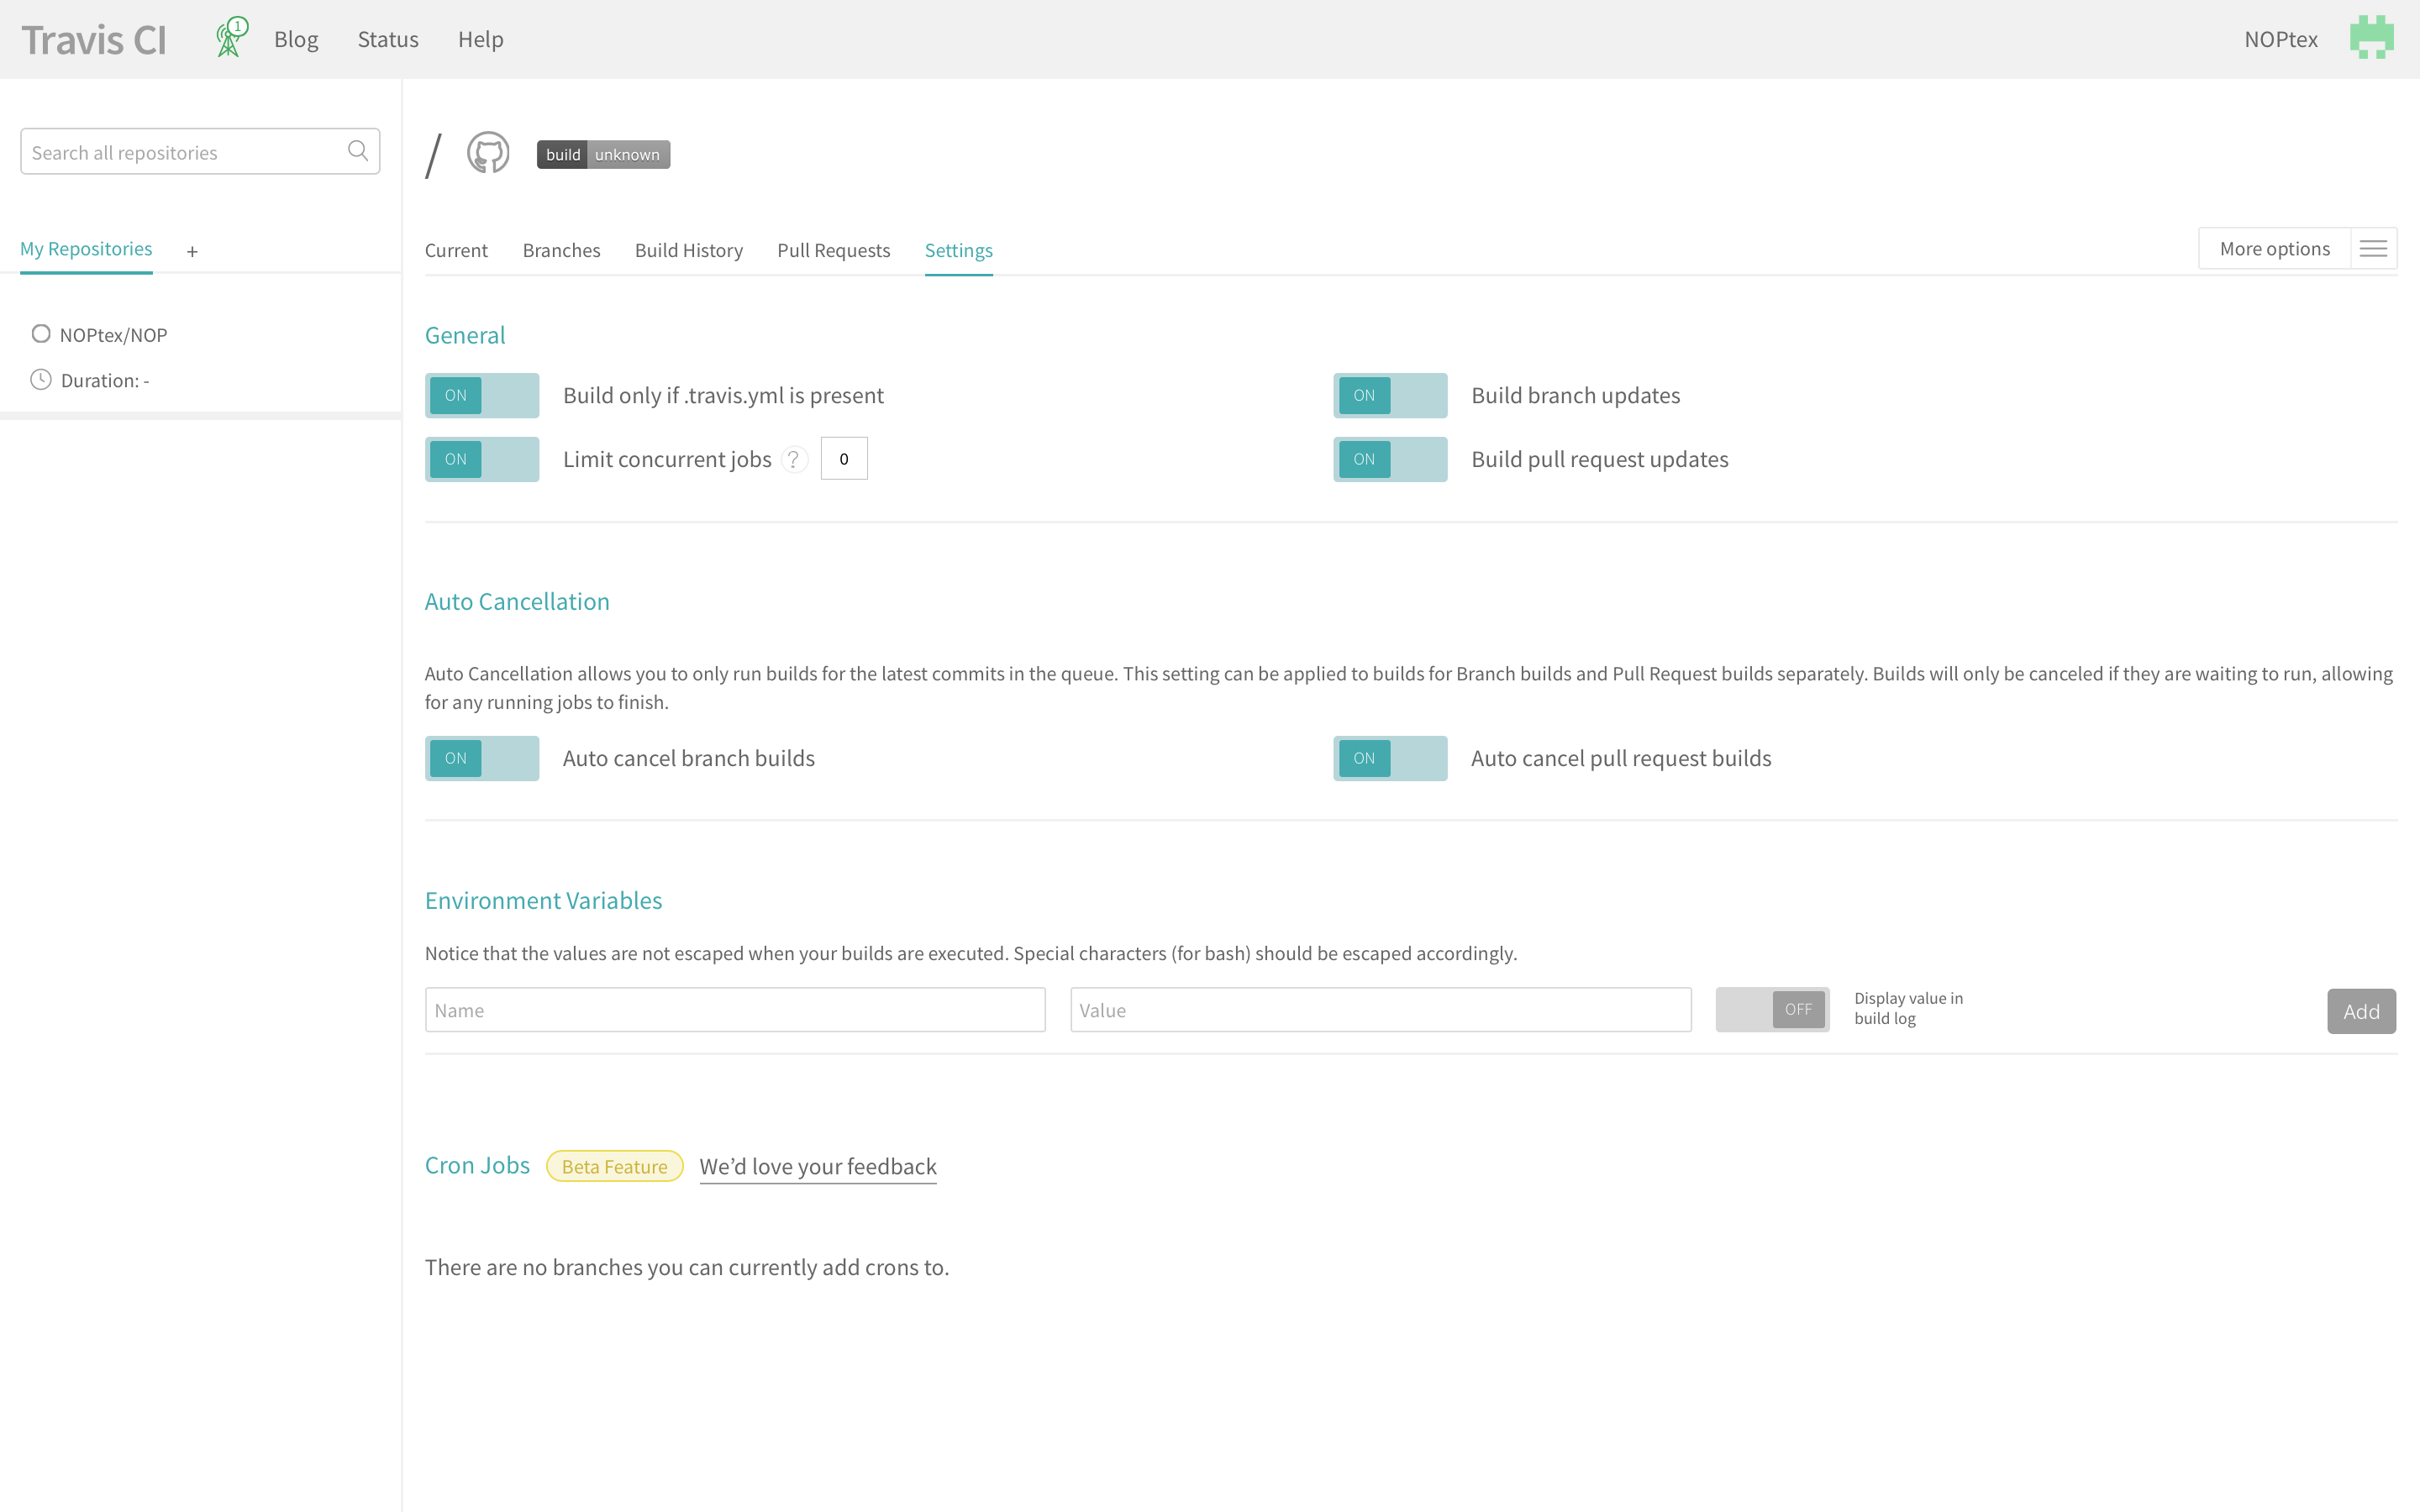
\includegraphics[width=1.0\textwidth]{./bilder/8TRAVISOptionsSET.png}
\end{framed}

\end{minipage}}
\hfill
\adjustbox{valign=t}{\begin{minipage}[t]{0.45\textwidth}
\vspace{0pt}
\huge
Ich setze alle Häkchen weil:
\begin{itemize}
  \item nur releases Gebaut werden sollen \\ (Testen kann man lokal) \\ Alle anderen Build sollen abgebrochen werden.
  \item Nur wenn .travis.yml vorhanden ist Build starten. \\(Einfaches deaktivieren über Git)
\end{itemize}
% \caption{Kapazität}
\end{minipage}}
\end{figure}

\clearpage % GleitObjekte anzeigen


%
% \newpage % ============================================= Newpage ===================
%
%
% \begin{figure}[ht]
%   \subsubsection{Build-Einstellungen setzen}
% \adjustbox{valign=t}{\begin{minipage}[t]{0.50\textwidth}
% \begin{framed}
%   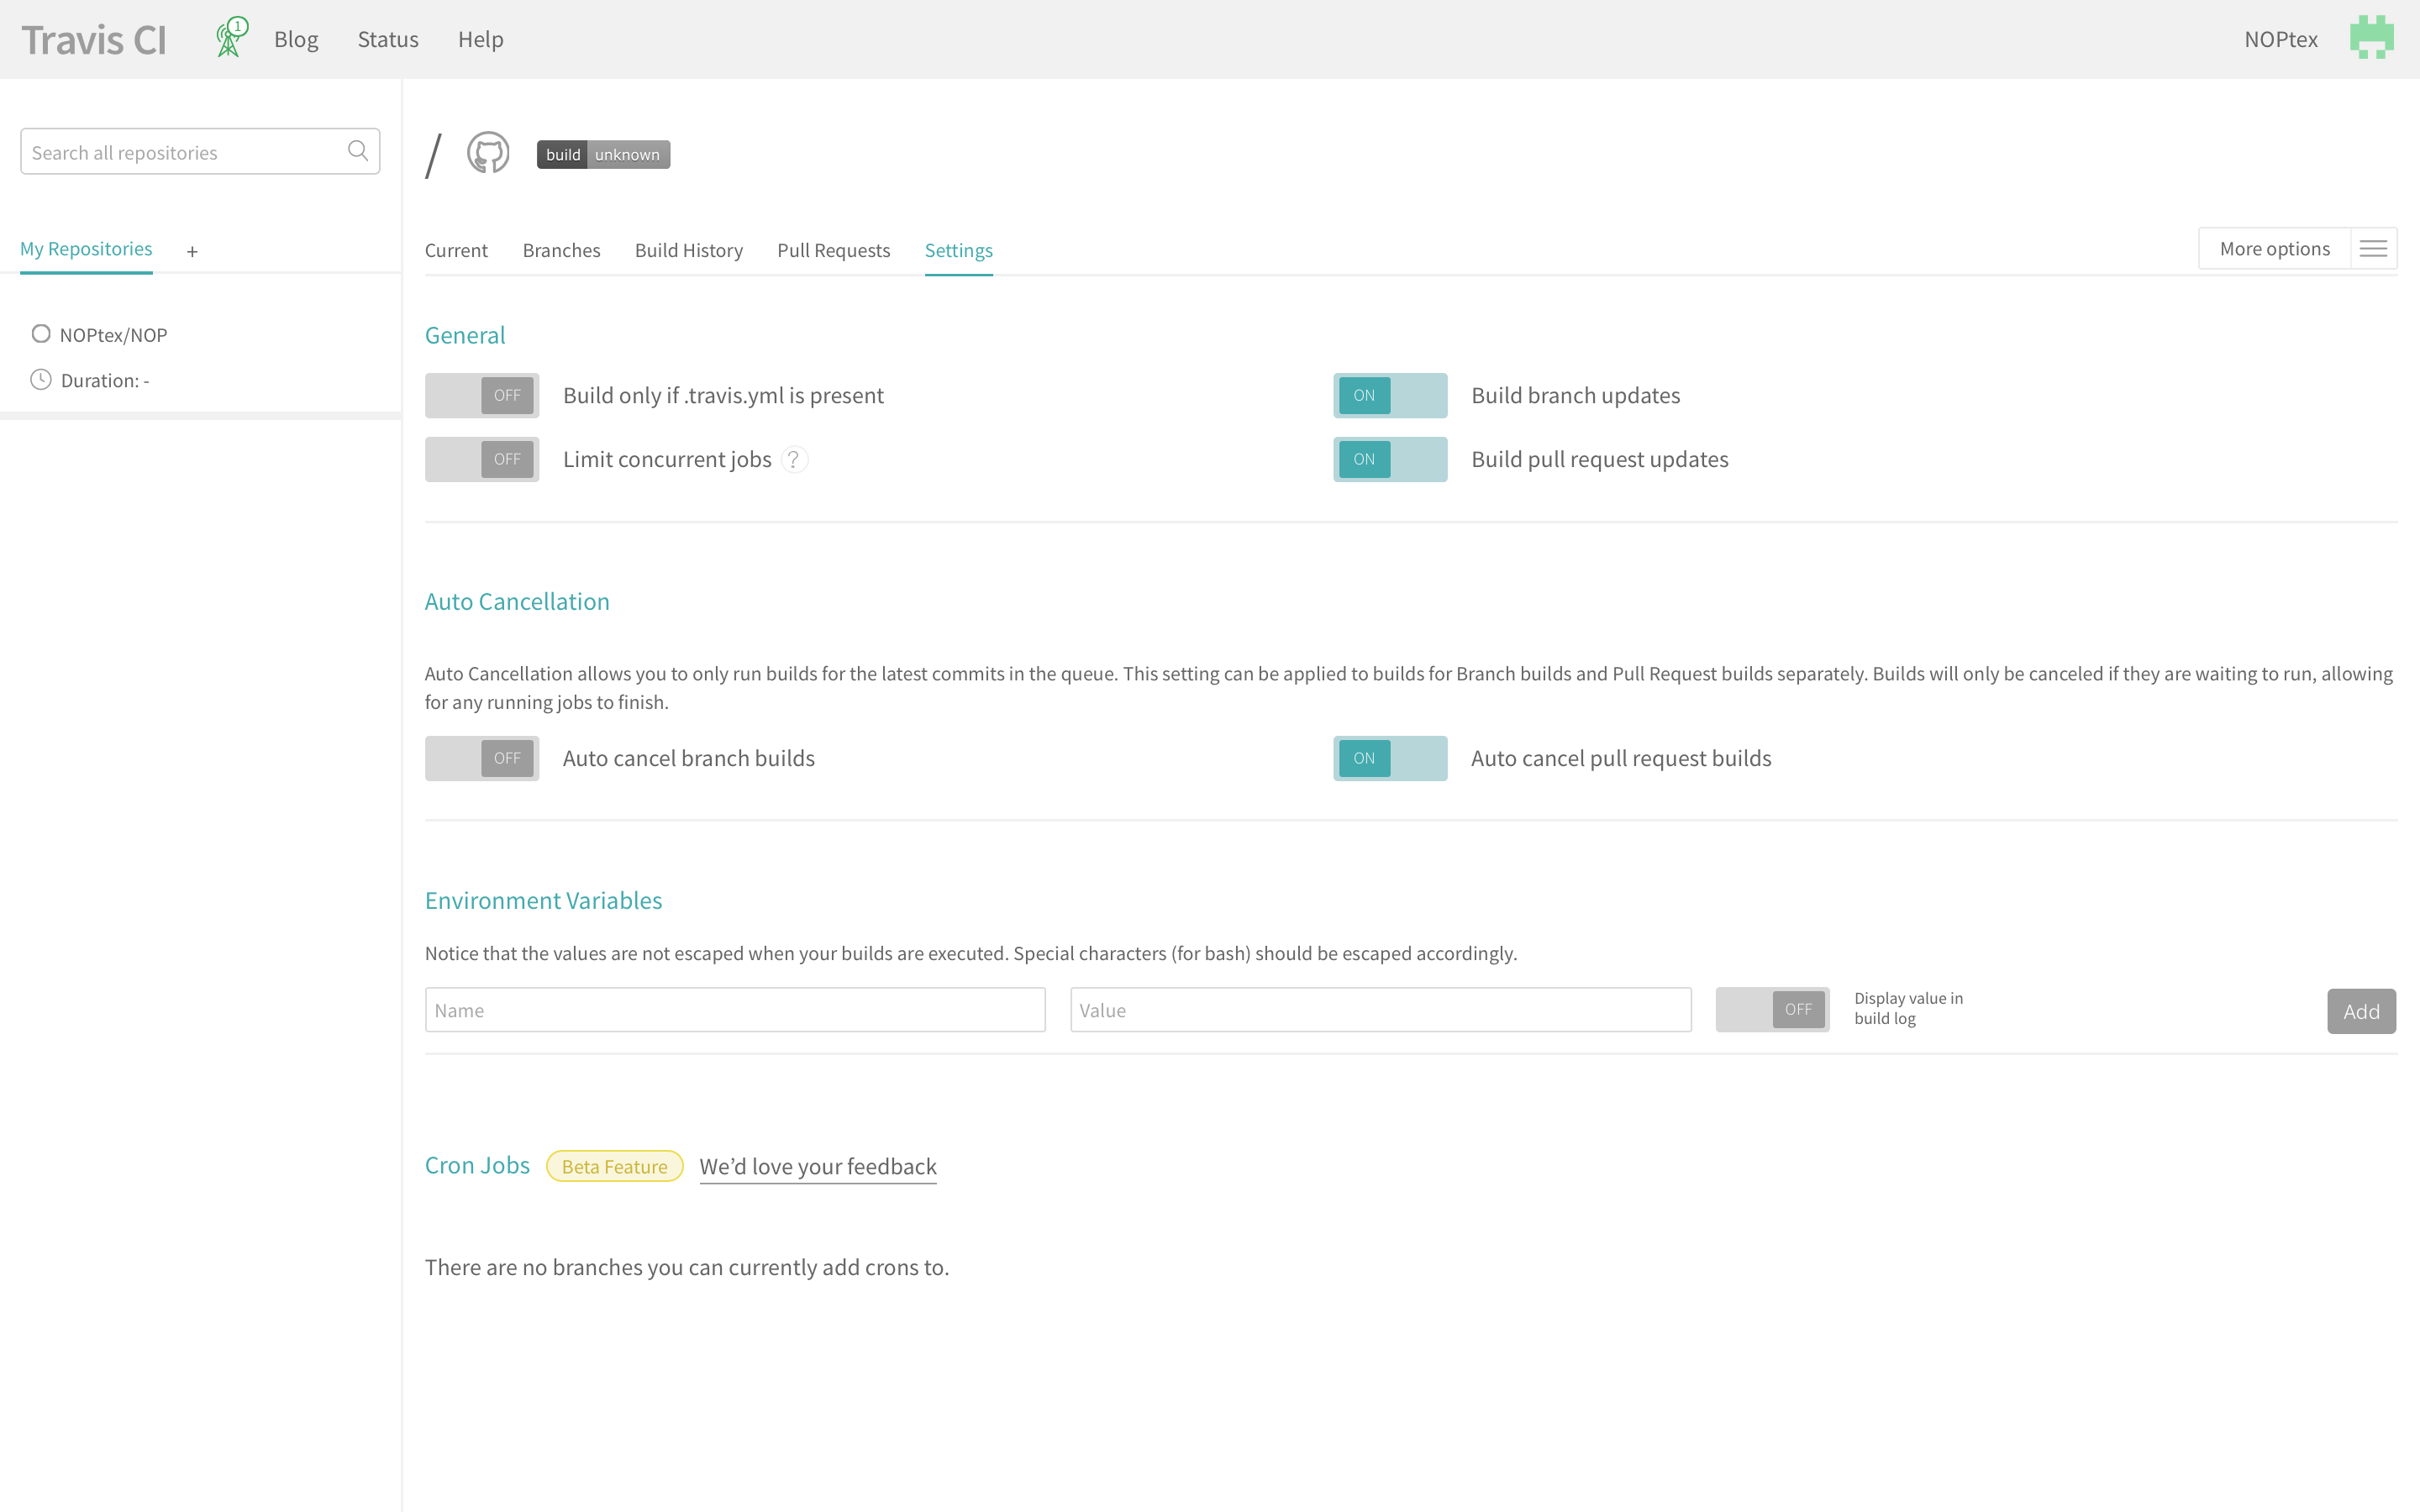
\includegraphics[width=1.0\textwidth]{./bilder/7TRAVISOptionsbase.png}
% \end{framed}
%
% \end{minipage}}
% % \hfill
% \adjustbox{valign=t}{\begin{minipage}[t]{0.45\textwidth}
% \vspace{0pt}
% 
\includegraphics[width=1.0\textwidth]{./bilder/7_1REPOsettings.png}
% \huge
% Über das Zahnrad kommt man zu den Einstellungen.
% % \caption{Kapazität}
% \end{minipage}}
% % \end{figure}
% % \vspace{0.5cm} % ----------------------------------- vspace
% % \begin{figure}[ht]
% \adjustbox{valign=t}{\begin{minipage}[t]{0.50\textwidth}
% % \vspace{0.5cm}
% \begin{framed}
%   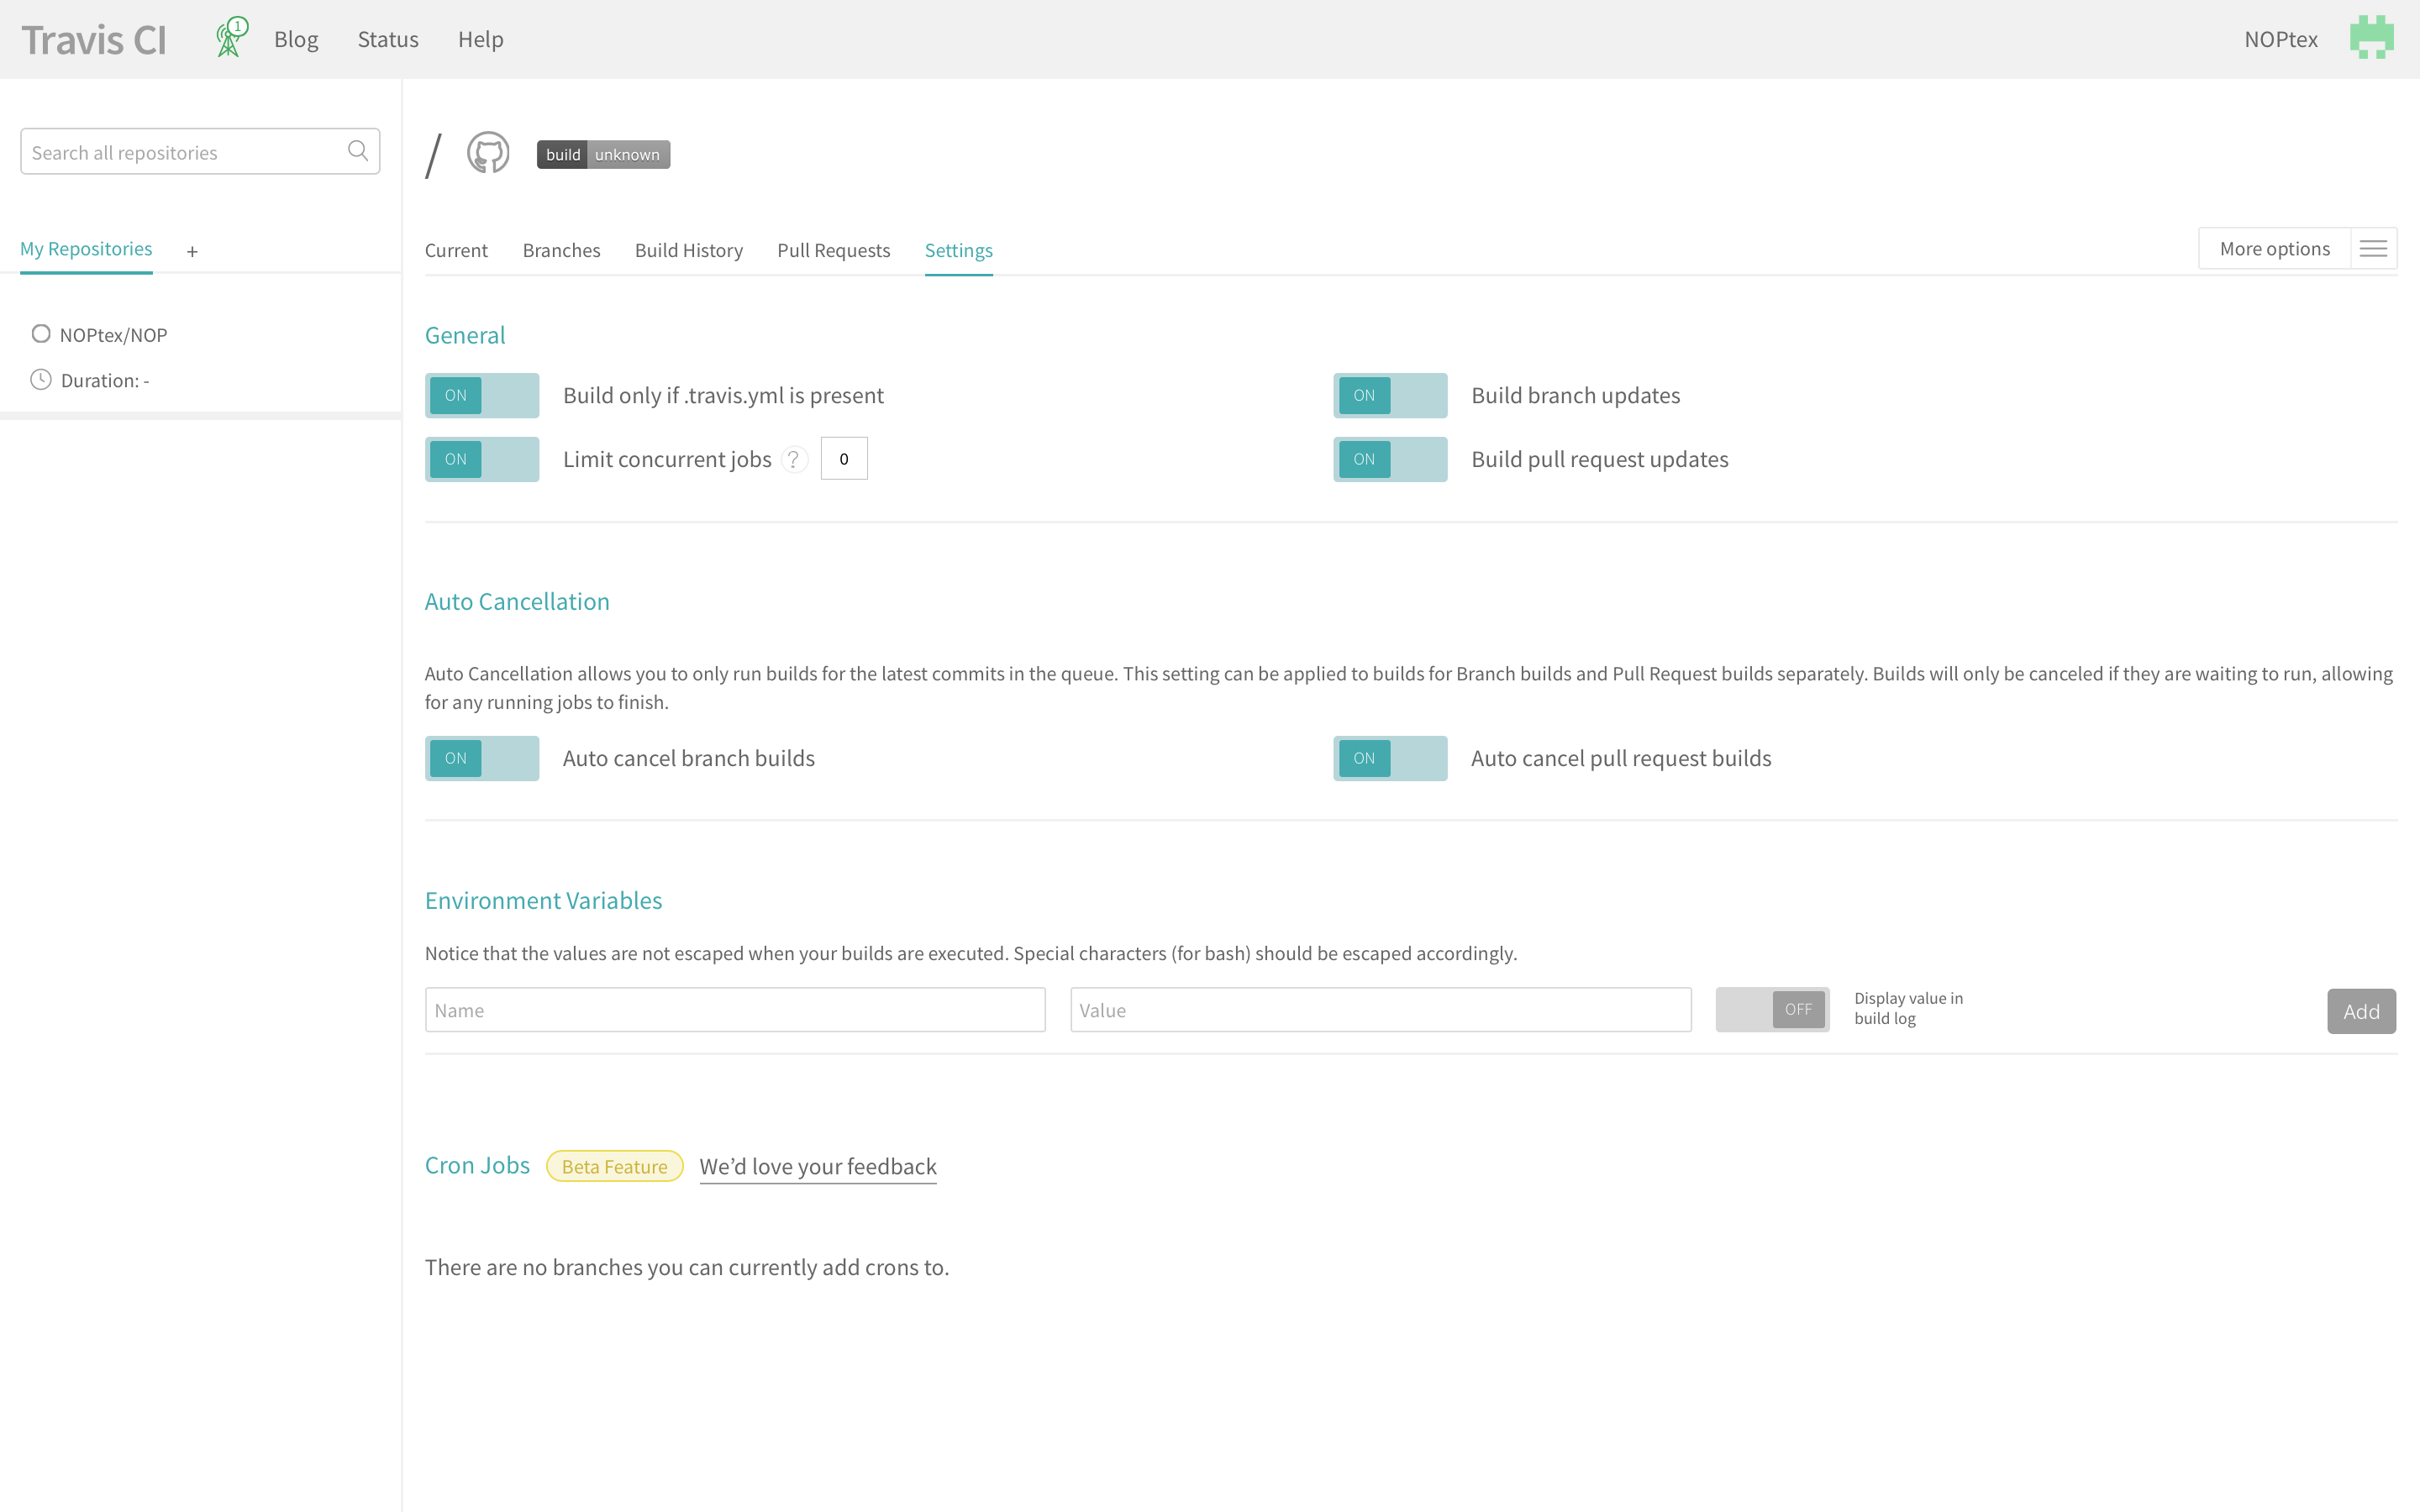
\includegraphics[width=1.0\textwidth]{./bilder/8TRAVISOptionsSET.png}
% \end{framed}
%
% \end{minipage}}
% \hfill
% \adjustbox{valign=t}{\begin{minipage}[t]{0.45\textwidth}
% \vspace{0pt}
% \huge
% Ich setze alle Häkchen weil:
% \begin{itemize}
%   \item nur releases Gebaut werden sollen \\ (Testen kann man lokal) \\ Alle anderen Build sollen abgebrochen werden.
%   \item Nur wenn .travis.yml vorhanden ist Build starten. \\(Einfaches deaktivieren über Git)
% \end{itemize}
% % \caption{Kapazität}
% \end{minipage}}
% \end{figure}
%
% \clearpage % GleitObjekte anzeigen




% \input{dummy.tex}
% \input{dummy.tex}
% \input{dummy.tex}
% \input{dummy.tex}

% \input{prog1.tex}



%  die beiden unteren beiden includen

% \input{kap1_vorl.tex}
% \input{kap2_vorl.tex}
% \input{kap3_vorl.tex}
% \input{kap4_vorl.tex}
% \input{kap5_vorl.tex}
% \input{kap6_vorl.tex}
% kapitel 7 im Buch

%   Kapitel 2

% \input{2ndKap7.tex}




%==============================================

% % programmieren 2

% \input{kap8.tex}
% \input{kap9.tex}
% \input{kap10.tex}
% \input{kap11.tex}
% \input{kap12.tex}
% \input{last.tex}
% \input{einfuerung.tex}




%=========================================================================================================================
%
%-------------END
\end{document}
